\chapter{The Standard Model of Particle Physics}

%\epigraph{\textit{So it goes...}}{---Kurt Vonnegut, \textit{Slaughterhouse
%		Five}}
	
%\epigraph{\textit{Science is a miracle.}}{--Ron Swanson}

\epigraph{\textit{If you wish to make an apple pie from scratch, you must first invent the universe.}}{--Carl Sagan, \textit{Cosmos: A Personal Voyage}}
\epigraph{\textit{All models are wrong, but some are useful.}}{--George Box}

As it stands, what has become known as the `Standard Model (SM) of Particle Physics'
is nothing less than one of the greatest achievements of mankind, due to both
the magnitude by which it has changed our perception of the underlying
nature of the universe and to the methods and tinkerings by which this
nature was unveiled by many clever physicists whose history has become veritable lore.
In terms of imagination and insight, it is second only to the special and general theories of relativity --
though the fields are nevertheless intricately intertwined.
%{\color{red}{The latter, though, being put forth by essentially a single person and the latter by a great many...}}.

Not considering the scientific progress made in the $18^{th}$ and $19^{th}$ centuries, and
ignoring the ancient Greeks despite their fabled invention of atomic theory,
the physical insights and major work that led to the current picture of elementary particle
physics described by the SM began with the \textit{annus mirabilis} papers of Albert
Einstein in the year 1905~\cite{einsteinPEE,einsteinSpecial,einsteinEnergyMass}.
In these papers, Einstein was able to shed light on the quantization of electromagnetic
radiation (building off of the seminal work of Max Planck~\cite{planckBlackBody})
and introduce the special theory of relativity.
These works laid the conceptual
and philosophical groundwork for the major breakthroughs in fundamental physics
of $20^{th}$ century physics: from the `old quantum theory' of Bohr and Sommerfeld
in the early 1900's to the equivalent wavefunction and matrix-mechanics formulations
of Schr{\"o}dinger and Heisenberg that
coalesced into `modern' quantum mechanics in the mid-1920's.
The modern approach, non-relativistic at its heart, provided a sufficient mathematical
and interpretable framework in which to work and match predictions to observed phenomena, old
and new. It has for the most part remained unchanged and is the quantum mechanics that is taught to
students at both the undergraduate and graduate level to this very day.
It is the theory that has since revolutionised all aspects of the physical sciences and
technologies that dictate our everyday-lives.
In the mid-1920's, however, despite
large efforts put forth by the forbears of modern quantum mechanics, the quantum-mechanical
world had yet to be made consistent with Einstein's theory of relativity --- a requirement
that must be met for all consistent physical theories of nature.
It was the insight of Paul Dirac who was finally able to successfully
marry the theory of the quantum with that of relativity when he introduced
his relativistic quantum-mechanical treatment of the electron in 1927 and 1928~\cite{diracEquation,Dirac:1927dy}.\footnote{
A complete history of the people and ideas involved in the development of the modern
theory of Quantum Mechanics can be found in references ~\cite{boffiRiseOfQM,historyQM},
and the references therein.
}
This work provided the starting point for a decades-long search of a consistent quantum-mechanical
and relativistic treatment of electrodynamics, known as \textit{quantum electrodynamics} (QED).
The search for QED ended at the end of the 1940's with the groundbreaking work of Dyson, Feynman, Schwinger, and Tomanaga~\cite{qedTomonaga,qedFeynman0,qedFeynman1,qedFeynman2,qedSchwinger0,qedSchwinger1,qedDyson0,qedDyson1} that introduced the covariant and gauge invariant
formulation of QED --- the first such relativistic quantum field theory (QFT).
QED allowed the physicists to make predictions that agreed with observation at unprecedented levels
of accuracy and has since led to the adoption of its language and mathematical toolkit as the
foundational framework in which to construct models that accurately describe nature.\footnote{
	For a complete discussion of the developments leading up to QED, see the fabulous
	book by S. Schweber~\cite{Schweber:1994qa}.	
}
The SM is no less than an ultimate conclusion of these works: a consistent set of relativistic
quantum field theories, using the language developed by Feynman et al.,
that describes essentially all aspects of the known particles and forces that make up the 
observed universe.

%%%%%%%%%%%%%%%%%%%%%%%%%%%%%%%%%%%%%%%%%%%
%%%%%%%%%%%%%%%%%%%%%%%%%%%%%%%%%%%%%%%%%%%
%% sub section describing SM particle content and lagrangian
%%%%%%%%%%%%%%%%%%%%%%%%%%%%%%%%%%%%%%%%%%%
%%%%%%%%%%%%%%%%%%%%%%%%%%%%%%%%%%%%%%%%%%%
\section{Particles and Forces}
\label{sec:sm_description}

There are four known fundamental forces at work in the universe: electromagnetism,
the weak interaction, the strong interaction, and gravity.
Our understanding of the existence of each of these forces
has essentially been arrived at empirically, with physicists following experimental
clues, and their basic behaviors deduced after long trials of effort.
The SM encompasses all of these forces except for gravity, which currently
is only described by the classical (i.e. not quantum) theory of geometrodynamics, or general
relativity.
The gravitational interaction is incredibly weak in comparison to the others, however, and
is not relevant to the types of particle interactions that we are currently
sensitive to in particle physics experiments.
Electromagnetism is by far the most familiar, as it is the force
most commonly experienced and is what is at work in our everyday life (reaction forces between
objects on tables and chairs, friction, wall-plugs, batteries, DNA structure, etc...) and is typically what
students are first presented with in their physics studies.
The weak force is responsible for things like radioactive decay,
which makes possible the process of nuclear $\beta$-decay and the nuclear
fission process that fuels the sun, for example. The strong force is what binds protons
and neutrons together, and thus is responsible for holding together most of the (ordinary) matter
in the universe.\footnote{`Ordinary' to distinguish from dark matter, for example.}

The forces mediate the interactions between the matter particles, which we use to deduce
their presence. The SM predicts fundamental, point-like particles that appear in two
general classes depending on whether they have integral spin ($\mathcal{S} \in [0,1,2,...)$) or half-integral
spin ($\mathcal{S} \in [1/2, 3/2, ...)$); the former are referred to as \textit{bosons} and the
latter as \textit{fermions}.
In the SM, the particles that are responsible for making up matter are all spin-$1/2$ fermions
and are either \textit{leptons} or \textit{quarks}; within each class
there are three generations (or families) that are essentially copies of the first.
The forces in the SM are interpreted as being mediated by spin-$1$ bosons, referred to as the 
\textit{gauge bosons}.
The leptons and quarks all experience the weak force, but only the quarks experience
the strong interaction. All electrically charged particles interact with the electromagnetic
interaction.

The particles of the SM are described as quantum fields whose dynamics are
described by the SM Lagrangian from which the equations of motions can be derived.
The particles, and by extension the SM Lagrangian that describes them, are found to be invariant under transformations of spacetime 
(space translations, rotations, Lorentz boosts) and three internal transformations described by unitary transformations: $\mathcal{P} \times$\SUthree$_C \times $ \SUtwo$_L \times$ \Uone$_{Y}$.
This is illustrated in Figure \ref{fig:sm_forces}. The strong force is described by a
local \SUthree~symmetry that acts only on the particles that have \textit{color charge}.
The term ``color'' arises from the fact that the color charge is found to exist
in three varieties which have been labelled as red (r), blue (b), or green (g), and due
to the fact that ``colorless'' states are formed when all three are combined (r+g+b), just
like with visible light that humans are familiar with, or when states are formed of color-anti-color
pairs (r+$\bar{\text{r}}$). For this reason, the QFT describing the strong force is called
Quantum \textit{Chromo}dynamics (QCD), and is mediated by eight \textit{gluons} (\fieldG).
The particles subject to the weak force are invariant under weak-isospin \SUtwo~transformations,
mediated by the three  \fieldW~bosons (\fieldWone, \fieldWtwo, \fieldWthree).
The \Uone~transformations, mediated by the \fieldB~boson, preserve weak-hypercharge, $Y$.
The \SUtwo~symmetry is respected only by the left-handed chiral
particles (leptons or quarks), with the right-handed chiral particles not participating.
There is additionally a single scalar (i.e. spin-0) field, the Higgs field, that is an \SUtwo~doublet, about which more will be described shortly.
The particle content thus described is presented in detail in Table \ref{tab:sm_content}.
The \SUtwo~left-handed chiral fields appear as doublets and are grouped in
and `up-down' pair (e.g. (\fieldUl, \fieldDl) or (\fieldEl, \fieldNuEl)) whereas the right-handed chiral fields,
living in the singlet representation of \SUtwo, do not (e.g. \fieldUr)). Note
that the SM does not allow for right-handed neutrinos (a term like \fieldNuR~does not appear).

\begin{figure}[!htb]
	\begin{center}
		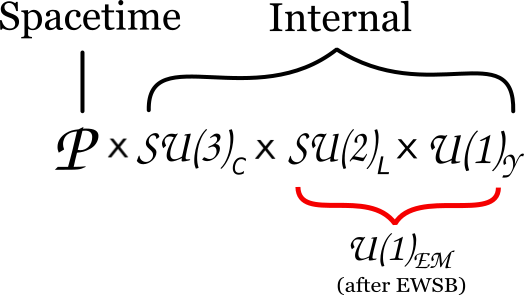
\includegraphics[width=0.5\textwidth]{figures/chapter1/sm_forces}
		\caption{
			The spacetime and internal gauge structure of the SM.
			$\mathcal{P}$ refers to the Poincar{\'e} symmetry group.
			\SUthree$_c$ refers to the \SUthree~symmetry
			of the color sector of QCD and \SUtwo$_{L}\times$\Uone$_{Y}$ refers to the left-handed chiral
			symmetry of the electroweak interaction. After spontaneous symmetry
			breaking due to the Higgs mechanism, the \SUtwo$_L \times$ \Uone$_Y$ symmetry
			reduces to the \Uone$_{EM}$ symmetry of electromagnetism. 
		}
		\label{fig:sm_forces}
	\end{center}
\end{figure}
\FloatBarrier

The SM Lagrangian is shown in Equation \ref{eq:sm_lagrangian} and describes the complete
content of the SM: encompassing all interactions between the known particles and the
symmetries that they obey.

\begin{align}
	\mathcal{L}_{\text{SM}} = -\frac{1}{4} \sum\limits_{\text{gauge}} \mathit{F}_{\mu \nu}^i \mathit{F}^{i\,\mu\nu}
	- \sum\limits_{f} \bar{f}\gamma^{\mu} \mathit{D}_{\mu} f 
	+  (\mathit{D}_{\mu} \phi)^{\dagger} (\mathit{D}^{\mu} \phi) - \mu^2 \phi^{\dagger}\phi - \lambda(\phi^{\dagger}\phi)^2
	\label{eq:sm_lagrangian}
\end{align}
\noindent
The first term of Equation~\ref{eq:sm_lagrangian} is a sum over the three internal gauge groups,  and $\mathit{F}^a_{\mu \nu} = \partial_{\mu} \mathit{A}_{\nu}^a - \partial_{\nu} \mathit{A}_{\mu}^a + g f^{abc} \mathit{A}_{\mu}^{b}\mathit{A}_{\nu}^{c}$, where $\mathit{A}_{\mu}$ is one of the
three gauge fields, $g$ is the associated gauge coupling parameter, and a sum over $i$ is implied. The $f^{abc}$ are the so-called
\textit{structure constants} of the gauge group. For Abelian groups like \Uone, $f^{abc}$ = 0.
For non-Abelian gauge groups like \SUtwo~and \SUthree, $f^{abc} \ne 0$. For example, for
\SUtwo~the structure constants are nothing more than the Levi-Civita totally anti-symmetric tensor, 
$\varepsilon_{ijk}$, giving for the weak gauge force:
\begin{equation}
	\mathbfcal{W}_{\mu \nu} = \partial_{\mu} \mathbfcal{W}_{\nu} - \partial_{\nu} \mathbfcal{W}_{\mu} - g_2 \mathbfcal{W}_{\mu} \times \mathbfcal{W}_{\nu}
\end{equation}
where $\mathbfcal{W}_{\mu}$ is the vector of the three weak gauge fields (\fieldWone, \fieldWtwo, and \fieldWthree) and $g_2$ is their associated gauge coupling. The non-zero $f^{abc}$ of non-Abelian gauge groups means that the gauge bosons of
the weak and strong interactions can interact with themselves due to terms appearing in Equation
\ref{eq:sm_lagrangian} that contain only the gauge bosons. %{\color{red}{add Feynman diagram? -- showing what the squared term of $W_{\mu \nu}$ representing triple and quartic couplings}}

The second term of Equation~\ref{eq:sm_lagrangian} describes the lepton and quark kinetic energies and their interactions with the gauge fields.
The $f$ refer to the fermion fields (quarks and leptons) and the corresponding sum is over all
species of fermion. $\mathit{D}_{\mu}$ is the gauge covariant derivative, and for the SM is
given by:

\begin{equation}
	\mathit{D}_{\mu} = \partial_{\mu} - i g_1 \frac{Y}{2} \mathcal{B}_{\mu} - i g_2 \frac{\tau^i}{2} \mathcal{W}_{\mu}^i - i g_3 \frac{\lambda^a}{2} G_{\mu}^a
	\label{eq:gauge_derivative}
\end{equation}
where $g_1$, $g_2$, and $g_3$ are the gauge coupling constants for \Uone$_{Y}$, \SUtwo$_{L}$, and \SUthree$_{C}$, respectively, that give the overall strength of the associated coupling.
Summation over repeated indices is implied and the $\tau^i$ ($\lambda^a$) are the three (eight)
generators of the \SUtwo~(\SUthree)~gauge group, with $i \in [1,2,3]$ ($a \in [1,..,8]$), and
are typically represented by the Pauli (Gell-Mann) matrices. Note that the form of Equation~\ref{eq:gauge_derivative} is strictly mandated by the requirement that the theory
be \textit{gauge invariant}, i.e. that transformations of the fields under the internal symmetries
of Figure \ref{fig:sm_forces} leave the action of $\mathcal{L}_{\text{SM}}$ unchanged. This is described in detail
in {\color{red}{Appendix XXX}}.

The last three terms in Equation \ref{eq:sm_lagrangian} are all terms including the Higgs field, $\phi$,
and will be discussed in detail in Section~\ref{sec:higgs_description}.

Inspection of Equation~\ref{eq:sm_lagrangian} will reveal two things. The first thing that one
may notice is that it does not appear to describe electromagnetism as it does not have a
term representing the photon, the familiar mediator of the electromagnetic interaction.
The second, and perhaps more immediately obvious, thing is that no mass terms
appear in $\mathcal{L}_{\text{SM}}$: all fields appear to have zero mass! Both of these
facts are counter to our everyday experience: we know electromagnetism is real and that matter,
at the very least, is massive. In the next few sections we will see how these apparent
issues are resolved.


\begin{table}[!htb]
    \caption{
        The particle content of the SM and their transformation
        properties under the SM gauge groups, prior to electroweak symmetry breaking.
        The representations of each of the gauge groups are shown in the three-right
        columns. The \Uone symmetry of weak-hypercharge transformations is one-dimensional
        and the column gives the weak-hypercharge $\mathcal{Y}$ associated with each
        field. For \SUthree and \SUtwo, $\mathbf{1}$ refers to the field belonging to
        the associated singlet representation, $\mathbf{2}$ to the doublet representation,
        $\mathbf{3}$ to the triplet representation, and $\mathbf{8}$ to the octet representation.
    }
    \begin{center}
        \begin{tabularx}{0.96\textwidth}{m{1em} c c c c c c }
        \toprule
        \hline
        & Field Label & Content & Spin & \Uone~($\mathcal{=Y}$) & \SUtwo & \SUthree \\
        \hline
        \rotatebox{90}{\hspace{-0.1cm}\textbf{Quarks} } 
         &   \makecell{\fieldQi \\ \fieldUri \\ \fieldDri} % FIELD
         &   \makecell{ (\fieldUl, \fieldDl), (\fieldCl, \fieldSl), (\fieldTl, \fieldBl) \\ \fieldUr \\ \fieldDr}% CONTENT
         &   \makecell{ $1/2$ \\ $1/2$ \\ $1/2$} % SPIN
         &   \makecell{ $1/6$ \\ $2/3$ \\ $-1/3$}% U(1)
         &   \makecell{ $\mathbf{2}$ \\ $\mathbf{1}$ \\ $\mathbf{1}$}% SU(2)
         &   \makecell{ $\mathbf{3}$ \\ $\mathbf{3}$ \\ $\mathbf{3}$}\\ % SU(3)
        %\cdashline{1-7}
        \rotatebox{90}{\hspace{-0.1cm}\textbf{Leptons} }
         &   \makecell{\fieldLi \\ \fieldEri} % FIELD
         &   \makecell{ (\fieldEl, \fieldNuEl), (\fieldMul, \fieldNuMul), (\fieldTaul, \fieldNuTaul) \\ \fieldEr, \fieldMur, \fieldTaur}% CONTENT
         &   \makecell{ $1/2$ \\ $1/2$ }% SPIN
         &   \makecell{ $1/2$ \\ $-1$ }% U(1)
         &   \makecell{ $\mathbf{2}$ \\ $\mathbf{1}$ }% SU(2)
         &   \makecell{ $\mathbf{1}$ \\ $\mathbf{1}$ } \\ % SU(3)
        \midrule
        \rotatebox{90}{\textbf{\stackanchor{Gauge}{Fields}} }
         &   \makecell{\fieldB \\ \fieldW \\ \fieldG } % FIELD
         &   \makecell{ \fieldB \\ (\fieldWone, \fieldWtwo, \fieldWthree) \\ \fieldG$_a$, $a\in[1,..,8]$ }% CONTENT
         &   \makecell{ $1$ \\ $1$ \\ $1$} % SPIN
         &   \makecell{ $0$ \\ $0$ \\ $0$}% U(1)
         &   \makecell{ $\mathbf{1}$ \\ $\mathbf{3}$ \\ $\mathbf{1}$}% SU(2)
         &   \makecell{ $\mathbf{1}$ \\ $\mathbf{1}$ \\ $\mathbf{8}$}\\ % SU(3)
        \midrule
        \rotatebox{90}{\textbf{\stackanchor{Higgs}{Field}}} 
         &   \makecell{\fieldPhi } % FIELD
         &   \makecell{ (\fieldPhip, \fieldPhizero) }% CONTENT
         &   \makecell{ $0$  } % SPIN
         &   \makecell{ $1/2$  }% U(1)
         &   \makecell{ $\mathbf{2}$ }% SU(2)
         &   \makecell{ $\mathbf{1}$ }\\ % SU(3)
        \hline
        \bottomrule
        \end{tabularx}
    \end{center}
    \label{tab:sm_content}
\end{table}

\FloatBarrier





%%%%%%%%%%%%%%%%%%%%%%%%%%%%%%%%%%%%%%%%%%%
%%%%%%%%%%%%%%%%%%%%%%%%%%%%%%%%%%%%%%%%%%%
%% sub section describing electroweak theory
%%%%%%%%%%%%%%%%%%%%%%%%%%%%%%%%%%%%%%%%%%%
%%%%%%%%%%%%%%%%%%%%%%%%%%%%%%%%%%%%%%%%%%%
\section{The Electroweak Theory}
\label{sec:ewk_description}

It was the work of Glashow, Weinberg, and Salam (GWS) that ultimately put forth a
consistent picture of the chiral weak force and
its unification with electromagnetism~\cite{Glashow:1961tr,Weinberg:1967tq,Salam:1968rm}.
As a result, the theory of particles and fields that respect the \SUewk~gauge
invariance of the SM is sometimes referred to as `GWS theory', 
but is more typically known as the electroweak theory. Since all matter particles
are subject to the electroweak interaction, but only a subset of the particles  that
have color charge (the quarks) are subject to the strong interaction described by QCD, the study of the SM can essentially
be partitioned into two parts: the part that deals with the dynamics and interactions of
colored objects (the `QCD part', $\mathcal{L}_{\text{QCD}}$) and the part that deals with electroweak
interactions, including the Higgs (the `Electroweak part`, $\mathcal{L}_{\text{Electroweak}}$).
Given the broad reach of the electroweak interaction,
in the early days GWS theory was considered the heart of the SM and why
GWS were awarded the Nobel prize in 1979.\footnote{Actually, the acceptance of the GWS theory as the
de-facto SM of the time was not widely held until some years after its publication, when t'Hooft
proved that it was renormalizable~\cite{tHooft:1971akt,tHooft:1971qjg}.
Such a complete understanding in the QCD sector would not come until almost a decade later, in the late
1970's{\color{red}{Woijkec etc CITE}}.}
In this section we will focus on the \SUewk~portion of \SML.

The first thing to remember is that the electroweak theory is \textit{chiral}, i.e., it distinguishes
between left- and right-chiral fermion fields.
For conceptual clarity, it is sometimes useful to take the massless (relativistic) limit of fermions to
get an idea of what chirality represents.
For a massless fermion field, the chirality is equivalent to the perhaps more-famility \textit{helicity},
defined as the projection of its spin onto its momentum (direction of motion).
The helicity of left-handed (right-handed) massless fermions is positive (negative), meaning
that its spin is parallel (anti-parallel) to its momentum.
Fermion fields, then, are commonly defined inclusive of their handedness, with the left-
and right-handed components projected out:
\begin{equation}
	f_{\text{L}} = P_L f = \frac{1}{2}(1- \gamma_5)f, \hspace{0.6cm} f_{\text{R}} = P_R f = \frac{1}{2}(1+\gamma_5)f
	\label{eq:chiral_projection}
\end{equation}

Let's focus only on the first generation of the leptons (the reasoning holds equally well
for the second and third generations, as well as for the quarks). Gathering the
\Uone terms of Eqn.~\ref{eq:sm_lagrangian} , we get Eqn.~\ref{eq:ferm_L_u1},
\begin{align}
    -\mathcal{L}_{\text{ferm}}(\mathcal{U}(1), \text{leptons}) &= \bar{L} i \gamma^{\mu} (i g_1 \frac{Y_L}{2} \mathcal{B}_{\mu})L + \bar{e}_R i \gamma^{\mu} (i g_1 \frac{Y_R}{2} B_{\mu}) e_R \nonumber \\
    &= \frac{g_1}{2} [ Y_L ( \bar{\nu}_L \gamma^{\mu} \nu_L + \bar{e}_L \gamma^{\mu} e_L) + Y_R \bar{e}_R \gamma^{\mu} e_R ] B_{\mu}
    \label{eq:ferm_L_u1}
\end{align}
Where $L = (\nu_L, e_L)$ is used in going from the first to second line. 
%Where we use the fact that $L = (\nu_L, e_L)$ in going from the first to second line of
%Eqn.~\ref{eq:ferm_L_u1}.
Likewise, gathering the associated \SUtwo~terms and noting that $\tau^i W^i$ is a
$2\times2$ matrix (the $\tau^i$ are the Pauli matrices),
%Gathering together the 
%Taking the associated \SUtwo~terms of Eqn.~\ref{eq:sm_lagrangian}, and noting
%that, since the $\tau^i$ are the Pauli matrices, $\tau^i W^i$ is a $2\times2$ matrix, we get:

\begin{equation}
	\begin{multlined}
		\hspace{-2cm}-\mathcal{L}_{\text{ferm}}(\mathcal{SU}(2), \text{leptons}) =  \bar{L}\, i \gamma^{\mu} [i g_2 \frac{\tau^i}{2} W_{\mu}^i ] \,L \\
		= -\frac{g_2}{2} \left[ \bar{\nu}_L \gamma^{\mu} \nu_L W_{\mu}^0 - \sqrt{2}  \bar{\nu}_L \gamma^{\mu} e_L W_{\mu}^+ - \sqrt{2} \bar{e}_L \gamma^{\mu} \nu_L W_{\mu}^- - \bar{e}_L \gamma^{\mu} e_L W_{\mu}^0 \right]
	\end{multlined}
	\label{eq:ferm_L_su2}
\end{equation}
Where we have used the following in Eqn.~\ref{eq:ferm_L_su2},
\begin{equation}
	W_{\mu}^+ = \frac{1}{\sqrt{2}} \left( -W_{\mu}^1 + i W_{\mu}^2 \right) \hspace{1cm} W_{\mu}^- = \frac{1}{\sqrt{2}} \left( -W_{\mu}^1 - i W_{\mu}^2 \right) \hspace{1cm} W_{\mu}^0 = W_{\mu}^3
\end{equation}

%\begin{align}
%	-\mathcal{L}_{\text{ferm}}(\mathcal{SU}(2), \text{leptons}) &= \bar{L} i \gamma^{\mu} [i g_2 \frac{\tau^i}{2} \mathcal{W}_{\mu}^i ] L \notag \\
%	&= -\frac{g_2}{2} (\bar{\nu}_L, \bar{e}_L) \gamma^{\mu} \left( \begin{matrix} \mathcal{W}_{\mu}^3 & \mathcal{W}_{\mu}^1 - i\mathcal{W}_{\mu}^2 \\ \mathcal{W}_{\mu}^1 + i \mathcal{W}_{\mu}^2  & - \mathcal{W}_{\mu}^3\end{matrix} \right) \left( \begin{matrix} \nu_L \\ e_L \end{matrix} \right) \notag \\
%	&= -\frac{g_2}{2} \left[ \bar{\nu}_L \gamma^{\mu} \nu_L \mathcal{W}_{\mu}^0 - \sqrt{2}  \bar{\nu}_L \gamma^{\mu} e_L \mathcal{W}_{\mu}^+ - \sqrt{2} \bar{e}_L \gamma^{\mu} \nu_L \mathcal{W}_{\mu}^- - \bar{e}_L \gamma^{\mu} e_L \mathcal{W}_{\mu}^0 \right]
%\end{align}
%Where Eqn.~\ref{eq:w_redefine} has been used in getting to the last line of Eqn.~\ref{eq:ferm_L_su2}.

Equations~\ref{eq:ferm_L_u1} and \ref{eq:ferm_L_su2} in principle describe all electroweak interactions
between matter and the gauge fields of \SUewk. We would like to make the correspondence
between these equations and what we know to empirically exist: the electromagnetic interaction
and the presence of a massive, charged mediator of the weak nuclear force responsible
for nuclear $\beta$-decay, for example. From the theory of QED, we know that the photon should
couple to charged objects and conserve electric charge. Inspecting all charge-preserving
terms of Eqn.~\ref{eq:ferm_L_u1} and \ref{eq:ferm_L_su2}, we note that we can perform
a field-redefinition,
\begin{equation}
	\left( \begin{matrix} A_{\mu} \\ Z_{\mu} \end{matrix} \right) = \left( \begin{matrix} \cos \theta_W & \sin \theta_W \\ -\sin \theta_W & \cos \theta_W \end{matrix} \right) \left( \begin{matrix} B_{\mu} \\ W_{\mu}^0 \end{matrix} \right)
\end{equation}
where we have used $Y_L = -1$ and introduce,
\begin{equation}
\sin \theta_W = \frac{g_1}{\sqrt{g_1^2 + g_2^2}} \hspace{1cm} \cos \theta_W = \frac{g_2}{\sqrt{g_1^2 + g_2^2}} \hspace{1cm} e = \frac{g_1 g_2}{\sqrt{g_1^2 + g_2^2}}
\label{eq:weinberg_angles}
\end{equation}
The angle $\theta_W$  is known as the \textit{Weinberg angle}. It quantifies the amount of
\textit{gauge mixing} that occurs between the neutral
\SUewk~gauge fields, \fieldB$_{\mu}$ and \fieldWzero$_{\mu}$.

Considering only those terms which are charge-neutral in Eqn.~\ref{eq:ferm_L_u1} and Eqn.~\ref{eq:ferm_L_su2}, one can consider performing a second field-redefinition using
\fieldB~ and \fieldWzero:
\begin{align}
	A_{\mu} &= \frac{g_2 \mathcal{B}_{\mu} - g_1 Y_L \mathcal{W}_{\mu}^0}{\sqrt{g_2^2 + g_1^2 Y_L^2}} \hspace{1cm} Z_{\mu} = \frac{g_1 Y_L \mathcal{B}_{\mu} + g_2 \mathcal{W}_{\mu}^0}{\sqrt{g_2^2 + g_1^2 Y_L^2}} \notag \\
	\hookrightarrow B_{\mu} &= \frac{g_2 A_{\mu} + g_1 Y_L Z_{\mu}}{\sqrt{g_2^2 + g_1^2 Y_L^2}} \hspace{1cm} \mathcal{W}_{\mu}^0 = \frac{-g_1 Y_L A_{\mu} + g_2 Z_{\mu}}{\sqrt{g_2^2 + g_1^2 Y_L^2}}
\end{align}
Using this last result for the re-defined \fieldB~and \fieldWzero~in terms the
fields $A_{\mu}$ and $Z_{\mu}$ to re-write the terms in Eqn.~\ref{eq:ferm_L_u1} and~\ref{eq:ferm_L_su2} involving $\bar{e}_{L,R} \gamma^{\mu} e_{L,R}$, allows
one to see that $A_{\mu}$ should correspond to the photon of electromagnetism if we fix,
\begin{align}
	-e = \frac{g_1 g_2 Y_L} {\sqrt{g_2^2 + g_1^2 Y_L^2}} \hspace{1cm} -e = \frac{g_1 g_2 Y_R}{2 \sqrt{g_2^2 + g_1^2 Y_L^2}} \nonumber
\end{align}
where $e$ is the charge of the positron. Setting $Y_L = -1$ then allows to formulate
the positron charge in terms of the weak couplings $g_1$ and $g_2$ simply as,
\begin{align}
	\label{eq:e_charge_coupling}
	e = \frac{g_1 g_2}{\sqrt{g_1^2 + g_2^2}}
\end{align}
Eqn.~\ref{eq:e_charge_coupling} leads one to introduce the following relations,
\begin{align}
	\sin \theta_W = \frac{g_1}{\sqrt{g_1^2 + g_2^2}} \hspace{1cm} \cos \theta_W = \frac{g_2}{\sqrt{g_1^2 + g_2^2}}
\end{align}
The angle $\theta_W$ is the \textit{Weinberg angle} {\color{red}{What is it's value? -- point to table}}, and it represents the amount of mixing
occuring between the \SUtwo~and \Uone~gauge fields $\mathcal{W}_{\mu}^0$ and $\mathcal{B}_{\mu}$, respectively. Using Eqn.~\ref{eq:e_charge_coupling} gives,
\begin{align}
	g_1 = \frac{e}{\cos \theta_W} \hspace{1cm} g_2 = \frac{e}{\sin \theta_W}
\end{align}
This defines the gauge couplings, $g_1$ and $g_2$, of the electroweak theory purely
in terms of known or measurable quantities.\footnote{We do not describe this in detail, but $\theta_W$
can in principle be determined once the masses of the $\mathcal{W^{\pm}}$ and $\mathcal{Z}$ bosons
are measured.}

From the above algebra, we can re-write the portion of the electroweak Lagrangian describing the
interactions of the first-generation fermions with the electroweak gauge bosons $A_{\mu}$,
$Z_{\mu}$, and $W^{\pm}$ as,
\begin{equation}
\begin{multlined}
\hspace{-0.9cm}\mathcal{L}_{\text{ferm, first-gen.}} = \underbrace{\sum\limits_{f \in \nu_e, e, u, d} e Q_f
\left(\bar{f}\gamma^{\mu} f \right) A_{\mu}}_\text{Neutral, $\sim$ EM}  \\
+ \underbrace{\frac{g_2}{\cos \theta_W} \sum\limits_{f \in \nu_e, e, u, d} \left[ \,\right.\bar{f}_L \gamma^{\mu} f_L
\left( T_f^3 -  Q_f \sin^2 \theta_W \right)
+ \bar{f}_R \gamma^{\mu} f_R \left(-Q_f \sin^2 \theta_W \right) \left. \right]\, Z_{\mu}}_\text{Neutral weak interaction} \\
+ \underbrace{\frac{g_2}{\sqrt{2}} \left[ \right. \left( \bar{u}_L \gamma^{\mu} d_L + \bar{\nu}_{e,L} \gamma^{\mu} e_L \right) \, W_{\mu}^+ + h.c. \left. \right]}_\text{Charged weak interaction}
\end{multlined}
\label{eq:ewk_L_za}
\end{equation}
%$\mathcal{L}_{\text{ferm, first-gen.}} = {\mathop{\sum}_\limits{f}} %_\limits{f \in \nu_e, e, u, d}} e Q_f% \left( %\bar{f}\gamma^{\mu} f \right) A_{\mu} \notag \\
%%	&+ {\mathop{\sum}_\limits{f \in \nu_e, e, u, d}} \frac{g_2}{\cos \theta_W} \left[ \bar{f}_L \gamma^{\mu} f_L \left( T_f^3 - Q_f \sin^2 \theta_W \right) + \bar{f}_R \gamma^{\mu} f_R \left( - Q_f \sin^2 \theta_W \right) \right] Z_{\mu} \label{eq:ewk_L_za} \\
%%	&+ \frac{g_2}{\sqrt{2}} \left[ \left( \bar{u}_L \gamma^{\mu} d_L + \bar{\nu}_L \gamma^{\mu} e_L \right) \mathcal{W}_{\mu}^+ + \text{hermitian conjugate} \right] \notag
%\end{multline}
The related terms for the second and third generations of the fermions,
($\nu_{\mu}, \mu, c, s$) and ($\nu_{\tau}, \tau, t, b$), respectively, are identical.
In Eqn.~\ref{eq:ewk_L_za}, $T_f^3$ ($Q_f$) is the third component of the weak-isospin (electric charge)
of the fermion species $f$. These last terms are related via the Gell-Mann-Nishijima relation,
\begin{align}
	Q_f = T_f^3 + \frac{1}{2}Y
	\label{eq:gell_mann_nishijima}
\end{align}
which can be deduced by following the algebra above, and our having fixed $Y_L = -1$ for
the $(\nu_L, e_L)$ \SUtwo~doublet.

Note that the terms involving \fieldWpm~in Eqn.~\ref{eq:ewk_L_za} are of the form $\bar{\nu}_L \gamma^{\mu} e_L$
which, given the chiral projects of Eqn.~\ref{eq:chiral_projection}, can be
re-written as follows,
\begin{align}
	\bar{\nu}_L \gamma{\mu} e_L = \frac{1}{2} \bar{\nu} \gamma^{\mu}(1-\gamma_5) e
	\label{eq:v_minus_a}
\end{align}
which shows that the charged weak interactions involving \fieldWpm~are the coherent
sum of vector ($\gamma^{\mu}$) and axial-vector ($\gamma^{\mu}\gamma_5$) bilinear covariants; this is the famous
\textit{V-A} charged-current interaction of Fermi's nuclear $\beta$-decay.
It is this \textit{V-A} form that results in the charged interactions of the weak force
not being invariant under chiral transformations ($f_R \leftrightarrow f_L$): it only involves
the left-chiral fermion fields. For this reason, \textit{parity}
is said to be maximally violated by the weak interaction.
This result, as presented in the above, is due to our having injected
it into our assumption on the field content in the first place out of hindsight. There
is no first-principles reason why the weak interactions should be this way, however,
and it was historically arrived at empirically.

What we have shown in this section is that, due to mixing of the SM \SUtwo$_L$
and \Uone$_Y$ gauge fields, we can arrive at an electroweak theory that supports
the known fact that their exists an electromagnetic force that is mediated
by a neutral boson $A_{\mu}$ (the photon) that couples to electrically charged fields: this is what
is shown in the first line of Eqn.~\ref{eq:ewk_L_za}. The field re-definitions described above
also introduce the \fieldWpm~boson as the mediators of the charged electroweak interaction,
responsible for radioactivity, and an additional neutral electroweak interaction mediated
by the \fieldZ~boson.
The fact that the \SUtwo$_L$ and \Uone$_Y$ gauge fields mix, by an amount dictated by $\theta_W$,
suggest that the weak and electromagnetic interactions can be unified into the single
electroweak interaction, as mentioned at the beginning of this section. Later on, we will see
that (gauge) unification such as this plays a large role in our current understanding
of how the universe works.

We have thus shown that the SM predicts the existence of the familiar electromagnetic force,
which is not immediately apparent based on \SML~of Eqn.~\ref{eq:sm_lagrangian}. 
%However, 
%neither the fermions nor the \fieldWpm~or \fieldZ~ appear to have mass -- they still
%have no mass terms appearing in their respective sectors of \SML.
However, it is still not evident how it can
support the experimental fact that fermions have mass and that the mediators of the
weak-nuclear force (the \fieldWpm) \textit{must} be massive given the very short
range of the interaction, a fact known
even before the formulation of QED. No such mass terms
have been provided for in the SM Lagrangian described by Eqn.~\ref{eq:sm_lagrangian}. To resolve this, we need the Higgs mechanism.


%%%%%%%%%%%%%%%%%%%%%%%%%%%%%%%%%%%%%%%%%%%
%%%%%%%%%%%%%%%%%%%%%%%%%%%%%%%%%%%%%%%%%%%
%% sub section describing the higgs mechanism
%%%%%%%%%%%%%%%%%%%%%%%%%%%%%%%%%%%%%%%%%%%
%%%%%%%%%%%%%%%%%%%%%%%%%%%%%%%%%%%%%%%%%%%
\section{The Higgs Mechanism and Electroweak Symmetry Breaking}
\label{sec:higgs_description}

The missing mass-terms for the fields in \SML~are provided by the
Brout-Englert-Higgs (BEH) mechanism~\cite{Englert:1964et,Higgs:1964ia,Higgs:1964pj}.
Before describing the specifics of the BEH mechanism, we should first describe the problem
of why \SML~doesn't support general mass terms for any of the fields in the first place.
That is, for example, why can't a fermion term like $m \bar{f} f$ exist in \SML?

Adding mass terms to \SML~for the fermions explicitly breaks the underlying \SUtwo~
gauge symmetry. This can be understood if we recognize the experimentally supported
fact that the left-handed fermions appear as \SUtwo~doublets and that the
right-handed fermions as singlets,
\begin{align}
	m\bar{f}f &= m \bar{f}(P_L + P_R)f \notag \\
				   &= m \bar{f} P_L P_L f + m \bar{f} P_R P_R f  	\label{eq:bad_fermion_mass_term}\\
				   &= m \left( \bar{f}_R f_L + \bar{f}_L f_R \right), \notag
\end{align}
where we have used identity relations of the projection operators $P_L$ and $P_R$ and the fact that $\bar{f}P_L = \bar{f}_R$ (and vice-versa). The last line of Equation~\ref{eq:bad_fermion_mass_term} involve terms
mixing \SUtwo~doublets with \SUtwo~singlets. Such a term is therefore not allowed if we wish to keep the \SUtwo~gauge symmetry intact.

Mass terms for the gauge bosons, of the form $m B_{\mu} B^{\mu}$, also do not work. For the Abelian \Uone~symmetry, for example, gauge invariance implies invariance of \SML~under transformations
of the form $B_{\mu}^{\prime} \rightarrow B_{\mu} - \partial_{\mu}\chi /g$. Such a mass term for
the gauge bosons is clearly not invariant under such a transformation. Even forgoing this fact,
adding such a term would quickly lead to non-renormalizable divergences appearing in the theory,
due to the longitudinal field components that appear in massive field propagators, rendering \SML~meaningless.

The BEH mechanism provides a way out of this problem. It refers to the introduction of a
spin-0 field, the Higgs field (Table \ref{tab:sm_content}), to the SM along with its corresponding interaction
terms to \SML: the last three terms of Equation~\ref{eq:sm_lagrangian}. The final two terms make up
what is referred to as the Higgs potential and can be expressed as,
\begin{align}
	V(\phi) = - \mu^2 \phi^2 - \lambda \phi^4
	\label{eq:higgs_potential}
\end{align}
The Higgs field is an \SUtwo~doublet and it can be seen that the interactions
described by Equation~\ref{eq:higgs_potential} respect \SUtwo~gauge symmetry.
If $\mu^2>0$, nothing all too interesting occurs and Equation~\ref{eq:higgs_potential} describes
a self-interacting, complex scalar field. If we take $\mu^2<0$, however, then the classical
potential described by Equation~\ref{eq:higgs_potential} has non-zero minima located at
$\phi = \pm v$ with $v = \sqrt{-\mu^2 / \lambda}$.
This is illustrated in Figure~\ref{fig:higgs_ewsb}. We see that the stable equilibrium point $\phi_0$
of the Higgs potential, the \textit{Higgs vacuum expectatin value} (vev), is not at $\phi = 0$
but at $v$,
\begin{align}
	\phi_0 = \frac{1}{\sqrt{2}} \left( \begin{matrix} 0 \\ v \end{matrix} \right)
	\label{eq:higgs_vev}
\end{align}
The choice of Equation~\ref{eq:higgs_vev} to represent the Higgs vacuum is motivated by
the requirement that the vacuum not be electrically charged --- a fact motivated very much
by experiment and everyday experience --- so the up-type \SUtwo~component of the Higgs field, $\phi^+$ (Table \ref{tab:sm_content}), is chosen to be zero for $\phi_0$. The choice of an
electrically neutral vacuum sets the rest of the \SUewk~structure of the complex Higgs field
since, by the Gell-Mann-Nishijima relation (Equation~\ref{eq:gell_mann_nishijima}) and charge
conservation,
a  neutral \SUewk~field should have down-type \SUtwo~quantum numbers and \Uone~hypercharge
$Y=1$,
\begin{align}
	Q = T_3 + \frac{1}{2}Y \rightarrow Q_{\phi_0} = -\frac{1}{2} + \frac{1}{2} \times 1 = 0.
	\label{eq:higgs_charge}
\end{align}

Note that Equation~\ref{eq:higgs_vev} states that only one component of the Higgs \SUtwo~doublet
attains a non-zero vev. This clearly means that the \SUtwo~gauge symmetry is not respected
by the choice of $\mu^2 < 0$ and that the electroweak \SUewk~symmetry is
\textit{spontaneously broken}.\footnote{A symmetry of a Lagrangian is said to be
	`spontaneously' broken if the Lagrangian of the underlying theory
	respects the symmetry but it gets broken through dynamical means or if the lowest-energy
	state (vacuum) does not respect the symmetry.
} The Higgs field
acquiring a non-zero vev is then referred to as the \textit{electroweak symmetry breaking} (EWSB) of the SM.

To further examine the physical consequences of EWSB,
we perturb the Higgs field about its minimum value,
\begin{align}
	\phi(x) \propto \left( \begin{matrix} 0 \\ \frac{1}{2}(v + h(x)) \end{matrix} \right),
	\label{eq:higgs_perturb}
\end{align}
where $h(x)$ correspond to excitations of the Higgs field that represent the physically observable
Higgs boson.
Inserting Equation~\ref{eq:higgs_perturb} into the $\mathit{D}_{\mu}\phi$ terms
of Equation~\ref{eq:sm_lagrangian}, one eventually works through the algebra and obtains,
\begin{align}
	\lvert\mathit{D}_{\mu} \phi(x)\rvert^2 = \frac{1}{8} v^2 g_2^2 \left[ \left( W^1_{\mu} \right)^2 +\left( W^2_{\mu} \right)^2 \right] 
		+ \frac{1}{8} v^2 \left( g_1 B_{\mu} - g_2 W_{\mu}^3 \right)^2.
	\label{eq:higgs_gauge_expand} 
\end{align}
Using the field re-definitions for the $W_{\mu}$, $A_{\mu}$ and $Z_{\mu}$ introduced in Section~\ref{sec:ewk_description}, we see that this can be re-written as (modulo factors of 2),
\begin{align}
	\lvert\mathit{D}_{\mu} \phi(x)\rvert^2 \propto \left(\frac{1}{2} v g_2 \right)^2 W_{\mu}^+ W^{-\,\mu} + \left( \frac{1}{2}v \sqrt{g_1^2 + g_2^2} \right)^2 Z_{\mu} Z^{\mu} + (0)^2 A_{\mu} A^{\mu},
	\label{eq:higgs_gauge_masses}
\end{align}
which provide, clearly, mass terms for the electroweak gauge bosons:
\begin{align}
	M_W = \frac{1}{2}v g_2, \hspace{1cm} M_Z = \frac{1}{2}v\sqrt{g_1^2 + g_2^2}, \hspace{1cm} M_A = 0.
	\label{eq:gauge_boson_masses}
\end{align}


The expression for the masses acquired by the \fieldWpm~and \fieldZ~gauge bosons in Equation~\ref{eq:gauge_boson_masses} is expected by Goldstone's theorem~\cite{Goldstone:1962es} which
states that for every broken continuous symmetry one expects an associated massless
scalar field (a `Goldstone boson') to appear in the theory. The fact that the \fieldWpm~and \fieldZ~acquire
mass after EWSB is then interpreted as these fields having acquired longitudinal field
components by `eating' the Goldstone boson degrees of freedom associated with the
breaking of \SUtwo$_L$. The BEH mechanism refers specifically to this means of the gauge
bosons acquiring mass via `eating' the Goldstone bosons.

The fact that the Higgs vev respects charge conservation (Equation~\ref{eq:higgs_charge}) means
that \SML, after EWSB, still respects a local \Uone~gauge symmetry; although now
this is the \Uone~gauge symmetry associated with electromagnetism, \Uone$_{EM}$,
as opposed to that of weak-hypercharge, \Uone$_Y$. This indicated in Figure~\ref{fig:sm_forces}.

There are also additional terms involving the now-massive \fieldWpm~and \fieldZ~ bosons and $h(x)$ in the expansion of $\lvert D_{\mu}\phi(x)\rvert^2$ of
Equation~\ref{eq:higgs_gauge_expand} (not shown) that describe the gauge bosons' interactions with the observable Higgs boson,
involving terms of the form $hVV$ and $hhVV$ ($V\in(W,Z)$) whose coupling strengths depend
on the gauge boson masses (Equation~\ref{eq:gauge_boson_masses}):
\begin{align}
	\mathcal{L}_{h-VV} \propto \frac{M_V^2}{v} \hspace{1cm} \mathcal{L}_{hh-VV} \propto \frac{M_V^2}{v^2}.
	\label{eq:higgs_gauge_couplings}
\end{align}
\begin{figure}[!htb]
	\begin{center}
		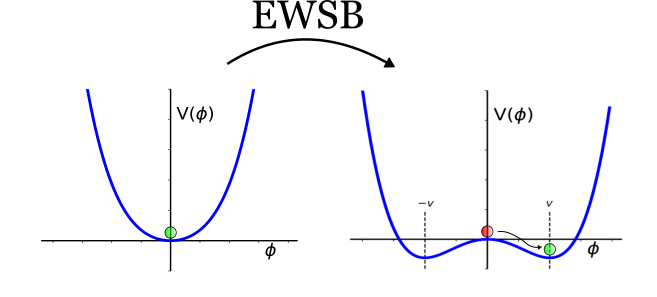
\includegraphics[width=0.75\textwidth]{figures/chapter1/higgs_potential_trans}
		\caption{Illustration of electroweak symmetry breaking (EWSB).
			\textbf{\textit{Left}}: Higgs potential with $\mu^2>0$ with stable equilibrium at $\phi=0$.
			\textbf{\textit{Right}}: With $\mu^2<0$, $\phi=0$ is no longer
			a stable equilibrium and the Higgs attains a non-zero vacuum
			expectation value at $\pm v$ --- breaking the \SUewk~gauge symmetry of the electroweak
			sector of the SM.
		}
	\label{fig:higgs_ewsb}
	\end{center}
\end{figure}

As opposed to `eating' gauge degrees of freedom as in the case of the \fieldWpm~and \fieldZ~bosons,
the fermion masses are obtained by adding additional interaction terms to \SML~between the
fermions and Higgs fields,
\begin{align}
	\mathcal{L}_{f-h} = y_f \left( \bar{L} \phi e^-_R + \phi^{\dagger} \overline{e^-}_R L\right).
	\label{eq:higgs_fermion_int}
\end{align}
Since both $L$ and $\phi$ are \SUtwo~doublets, adding the right-handed \SUtwo~singlet terms
do not spoil the \SUtwo~symmetry.
When the Higgs field acquires a non-zero vev after EWSB, we can insert Equation~\ref{eq:higgs_perturb} into Equation~\ref{eq:higgs_fermion_int} to obtain expressions for the fermions masses,
\begin{align}
	m_f = y_f \frac{v}{\sqrt{2}},
	\label{eq:fermion_mass_term}
\end{align}
where the $y_f$ are referred to as the fermion \textit{Yukawa couplings}, and are free parameters
of the SM that need to be measured.
Additional interactions arise between the fermions and $h(x)$ whose couplings are related
to the fermion masses as,
\begin{align}
	\mathcal{L}_{f-h} \propto \frac{m_f}{v} \bar{f}f h.
	\label{eq:higgs_fermion_coupling}
\end{align}

The general form Equation~\ref{eq:higgs_fermion_int} implies that the $y_f$ are matrices representing the
Higgs-fermion Yukawa couplings. They can be diagonalized by performing the proper unitary
transformations between the weak- and mass-bases of the fermion fields. In the case of the leptons,
this rotation is the identity: the lepton's weak eigenbasis is the same as their mass eigenbasis.
This is mainly due to the extraordinarily large mass difference between the charged and neutral
leptons within each lepton generation~\cite{Akhmedov:2007fk}. Within the quark-sector,  however,
the mass- and weak-basis fermion fields differ. This implies that the diagonalization procedure results
in mixing among the weak eigenstates of the quark fields to produce the observed mass eigenstates; i.e. the quark mass-eignstates ($d$,
$s$, $b$) are
coherent mixtures of the weak eigenstates ($d^{\prime}$,
$s^{\prime}$, $b^{\prime}$).\footnote{The mixing can be parametrised as either occurring between
the up-type, down-type, or a mixture of up- and down-type fields of each \SUtwo~doublet. Without
loss of generality and for simplicity, it is usually given with respect to the down-type quark fields as shown
here.}
This allows for the flavor-changing processes that are present
in charged weak interactions, allowing for interaction terms involving the decay
of a quark of one family into that of another family. The amount of mixing in the quark sector
is dictated by a $3\times 3$ unitary matrix known as the \textit{Cabibbo-Kobayashi-Maskawa} (CKM)
matrix~\cite{Kobayashi:1973fv} $\mathcal{V}_{\text{CKM}}$, the general form of which has four free parameters: three mixing angles
and a complex phase, $\delta$. The off-diagonal terms of the CKM matrix and the value of the mixing angles
dictate the amount of flavor mixing in the quark sector. The complex phase $\delta$
allows for charge-parity (CP) symmetry violating effects to occur. In fact, this term is the \textit{only} term of the SM
that allows for CP-violation --- an effect important for providing interactions that are asymmetric
between matter and anti-matter fields.\footnote{Charge Parity (CP) symmetry refers to the invariance
	of a theory with respect to swapping particles with their corresponding anti-particles and, additionally,
	inverting a field's spatial coordinates, $\psi(\vec{x}) \rightarrow \psi(-\vec{x})$. The former
	is the `C' symmetry and the latter is the `P' symmetry.
}

The remaining terms of $V(\phi)$ (Equation~\ref{eq:higgs_potential}) involve only the Higgs field. After
EWSB and the Higgs field acquiring vev we obtain,
\begin{align}
	V(\phi) \rightarrow V(\phi)_{\text{EWSB}} =  -\lambda \nu^2 h^2 - \lambda \nu h^3 - \frac{1}{4} \lambda h^4 + \text{const.}
	\label{eq:higgs_potential_self_int}
\end{align}
where we have ignored the terms already discussed above. The first term of Equation~\ref{eq:higgs_potential_self_int}
is the Higgs boson mass term, the second and third are the triple and quartic Higgs self-couplings,
\begin{align}
	\underbrace{m_{h} = \sqrt{ - 2 \mu^2} = \sqrt{ 2 \lambda v^2 }}_\text{Higgs boson mass} \hspace{1cm} \underbrace{\mathcal{L}_{hhh} \propto \frac{m_h^2}{v} \hspace{1cm} \mathcal{L}_{hhhh} \propto \frac{m_h^2}{v^2}}_\text{Triple and quartic Higgs self-couplings}.
	\label{eq:higgs_self_couplings}
\end{align}





%%%%%%%%%%%%%%%%%%%%%%%%%%%%%%%%%%%%%%%%%%%
%%%%%%%%%%%%%%%%%%%%%%%%%%%%%%%%%%%%%%%%%%%
%% sub section describing the standard model finally and its successes
%%%%%%%%%%%%%%%%%%%%%%%%%%%%%%%%%%%%%%%%%%%
%%%%%%%%%%%%%%%%%%%%%%%%%%%%%%%%%%%%%%%%%%%
\section{The Complete Standard Model, Successes and Shortcomings}
\label{sec:final_sm_description}

The physical field content of the SM, after EWSB, is detailed in Table~\ref{tab:sm_content_EWSB}
Also shown in Table~\ref{tab:sm_content_EWSB} are the electric charge associated with each
particle field, $Q$, the relevant couplings, and particle masses.


\begin{table}[!htb]
    \caption{
        The particle content of the SM after the process of
        electroweak symmetry breaking.
    }
    \begin{center}
        \begin{tabularx}{1\textwidth}{m{1em} c c c c }
        \toprule
        \hline
        & Physical Field & Q & Coupling & Mass [GeV] \\
        \hline
        \rotatebox{90}{\hspace{-0.1cm}\textbf{Quarks} } 
            & \makecell{ \quarkU, \quarkC, \quarkT \\ \quarkD, \quarkS, \quarkB} % FIELD
            & \makecell{ $2/3$ \\ $-1/3$ }% Q
            %& \makecell{ $\mathbf{3}$ \\ $\mathbf{3}$ } % SU(3)
            & \makecell{ ($y_i=$) $1\times10^{-5}$, $7\times10^{-3}$, $1$ \\ ($y_i=$) $3\times10^{-5}$, $5\times10^{-4}$, $0.02$ } % Coupling
            & \makecell{ $2\times10^{-3}$, $1.27$, $173$ \\ $4\times10^{-4}$, $0.10$, $4.18$ }\\% Mass
        \rotatebox{90}{\hspace{-0.1cm}\textbf{Leptons} } 
            & \makecell{ \leptonE, \leptonMu, \leptonTau \\ \neutrinoE, \neutrinoMu, \neutrinoTau } % FIELD
            & \makecell{ $-1$ \\ $0$ }% Q
            %& \makecell{ $\mathbf{1}$ \\ $\mathbf{1}$ } % SU(3)
            & \makecell{ ($y_i=$) $3\times10^{-7}$, $6\times10^{-4}$, $0.01$ \\ -- } % Coupling
            & \makecell{ $5\times10^{-4}$, $0.106$, $1.777$ \\ --}\\% Mass
        \midrule
        \rotatebox{90}{\textbf{Bosons} } 
            & \makecell{ \fieldPhoton \\ \fieldZ \\ (\fieldWp, \fieldWm) \\ \fieldG } % FIELD
            & \makecell{ $0$ \\ $0$ \\ $(+1,-1)$ \\ $0$ }% Q
            %& \makecell{ $\mathbf{1}$ \\ $\mathbf{1}$ \\ $\mathbf{1}$ \\ $\mathbf{8}$ } % SU(3)
            & \makecell{ $\alpha_{\text{EM}} \simeq 1/137$ \\ $\sin \theta_{W} \simeq 0.5$ \\ -- \\ $\alpha_s \simeq 0.1$ } % Coupling
            & \makecell{ $0$ \\ $91.2$ \\ $80.4$ \\  $0$}\\% Mass
        \midrule
        \rotatebox{90}{\textbf{Higgs} } 
            & \makecell{ \fieldH } % FIELD
            & \makecell{ $0$ }% Q
            %& \makecell{ $\mathbf{1}$ } % SU(3)
            & \makecell{ $\lambda$, $\mu$ } % Coupling
            & \makecell{ $125.09$ }\\% Mass

         %&   \makecell{ (\quarkUl, \quarkDl), (\quarkCl, \quarkSl), (\quarkTl, \quarkBl) \\ \quarkUr \\ \quarkDr}% CONTENT
         %&   \makecell{ $1/2$ \\ $1/2$ \\ $1/2$} % SPIN
         %&   \makecell{ $\mathbf{2}$ \\ $\mathbf{1}$ \\ $\mathbf{1}$}% SU(2)
         %&   \makecell{ $\mathbf{3}$ \\ $\mathbf{3}$ \\ $\mathbf{3}$}\\ % SU(3)
        %%\cdashline{1-7}
        %rotatebox{90}{\hspace{-0.1cm}\textbf{Leptons} }
         %&   \makecell{\quarkLi \\ \quarkEri} % FIELD
         %&   \makecell{ (\quarkEl, \quarkNuEl), (\quarkMul, \quarkNuMul), (\quarkTaul, \quarkNuTaul) \\ \quarkEr, \quarkMur, \quarkTaur}% CONTENT
         %&   \makecell{ $1/2$ \\ $1/2$ }% SPIN
         %&   \makecell{ $\mathbf{2}$ \\ $\mathbf{1}$ }% SU(2)
         %&   \makecell{ $\mathbf{1}$ \\ $\mathbf{1}$ } \\ % SU(3)
        %midrule
        %rotatebox{90}{\textbf{\stackanchor{Gauge}{Fields}} }
         %&   \makecell{\quarkB \\ \quarkW \\ \quarkG } % FIELD
         %&   \makecell{ \quarkB \\ (\quarkWone, \quarkWtwo, \quarkWthree) \\ \quarkG }% CONTENT
         %&   \makecell{ $1$ \\ $1$ \\ $1$} % SPIN
         %&   \makecell{ $\mathbf{1}$ \\ $\mathbf{3}$ \\ $\mathbf{1}$}% SU(2)
         %&   \makecell{ $\mathbf{1}$ \\ $\mathbf{1}$ \\ $\mathbf{8}$}\\ % SU(3)
        %midrule
        %rotatebox{90}{\textbf{\stackanchor{Higgs}{Field}}} 
         %&   \makecell{\quarkPhi } % FIELD
         %&   \makecell{ (\quarkPhip, \quarkPhizero) }% CONTENT
         %&   \makecell{ $0$  } % SPIN
         %&   \makecell{ $\mathbf{2}$ }% SU(2)
         %&   \makecell{ $\mathbf{1}$ }\\ % SU(3)
        \hline
        \bottomrule
        \end{tabularx}
    \end{center}
    \label{tab:sm_content}
\end{table}


%%%%%%%%%%%%%%%%%%%%%%%%%%%%%%%%%%%%%%%%%%%%%%%%%%%%%%%%%%%%%%%%%%%%%%%%%%%%%%%%%
%%%%%%%%%%%%%%%%%%%%%%%%%%%%%%%%%%%%%%%%%%%%%%%%%%%%%%%%%%%%%%%%%%%%%%%%%%%%%%%%%
%%%%%%%%%%%%%%%%%%%%%%%%%%%%%%%%%%%%%%%%%%%%%%%%%%%%%%%%%%%%%%%%%%%%%%%%%%%%%%%%%
%
% SUCCESSES
%
%%%%%%%%%%%%%%%%%%%%%%%%%%%%%%%%%%%%%%%%%%%%%%%%%%%%%%%%%%%%%%%%%%%%%%%%%%%%%%%%%
%%%%%%%%%%%%%%%%%%%%%%%%%%%%%%%%%%%%%%%%%%%%%%%%%%%%%%%%%%%%%%%%%%%%%%%%%%%%%%%%%
%%%%%%%%%%%%%%%%%%%%%%%%%%%%%%%%%%%%%%%%%%%%%%%%%%%%%%%%%%%%%%%%%%%%%%%%%%%%%%%%%

\subsection{Successes of the Standard Model}
\label{sec:sm_successes}

The particle content presented in Table~\ref{tab:sm_content_EWSB} represents the current
picture of the visible matter content of the Universe.
It is a concise picture.
With this particle content in hand, and the description of their fundamental particle interactions (Equation~\ref{eq:sm_lagrangian}, after EWSB),
the predictive power of the SM is immense.

Figure~\ref{fig:sm_xsec_summary} shows a summary of LHC measurements of cross-sections
for various production processes at 7, 8, and 13\,TeV.
The agreement of these measurements with the theoretical predictions provided by the SM, spanning over 10 orders of magnitude,
is an incredible testament to the power of the SM and the toolkit provided by QFT.
The power of the SM, and its internal consistency, is illustrated in Figure~\ref{fig:mw_mt_scan},
which shows the results of indirect measurements of the $W$-boson and top-quark masses based
on fits to electroweak precision data.
When all measurements other than those on $m_h$ are included, the constraints of the SM
only allow for a small region of the $(m_{\text{top}}, M_W)$ parameter space.
Adding the Higgs mass measurement results only shrinks this allowed area.
The fact that these indirect measurements agree so well with the direct measurements paints a picture
of the SM as being a fundamentally complete picture of the known physical phenomena.
It is likely that if the SM were not accounting for particular types of interactions or fields,
the level of agreement between the direct measurements and those obtained indirectly via
fits to electroweak precision data would not be to the level seen in Figure~\ref{fig:mw_mt_scan}.

\begin{figure}[!htb]
    \begin{center}
        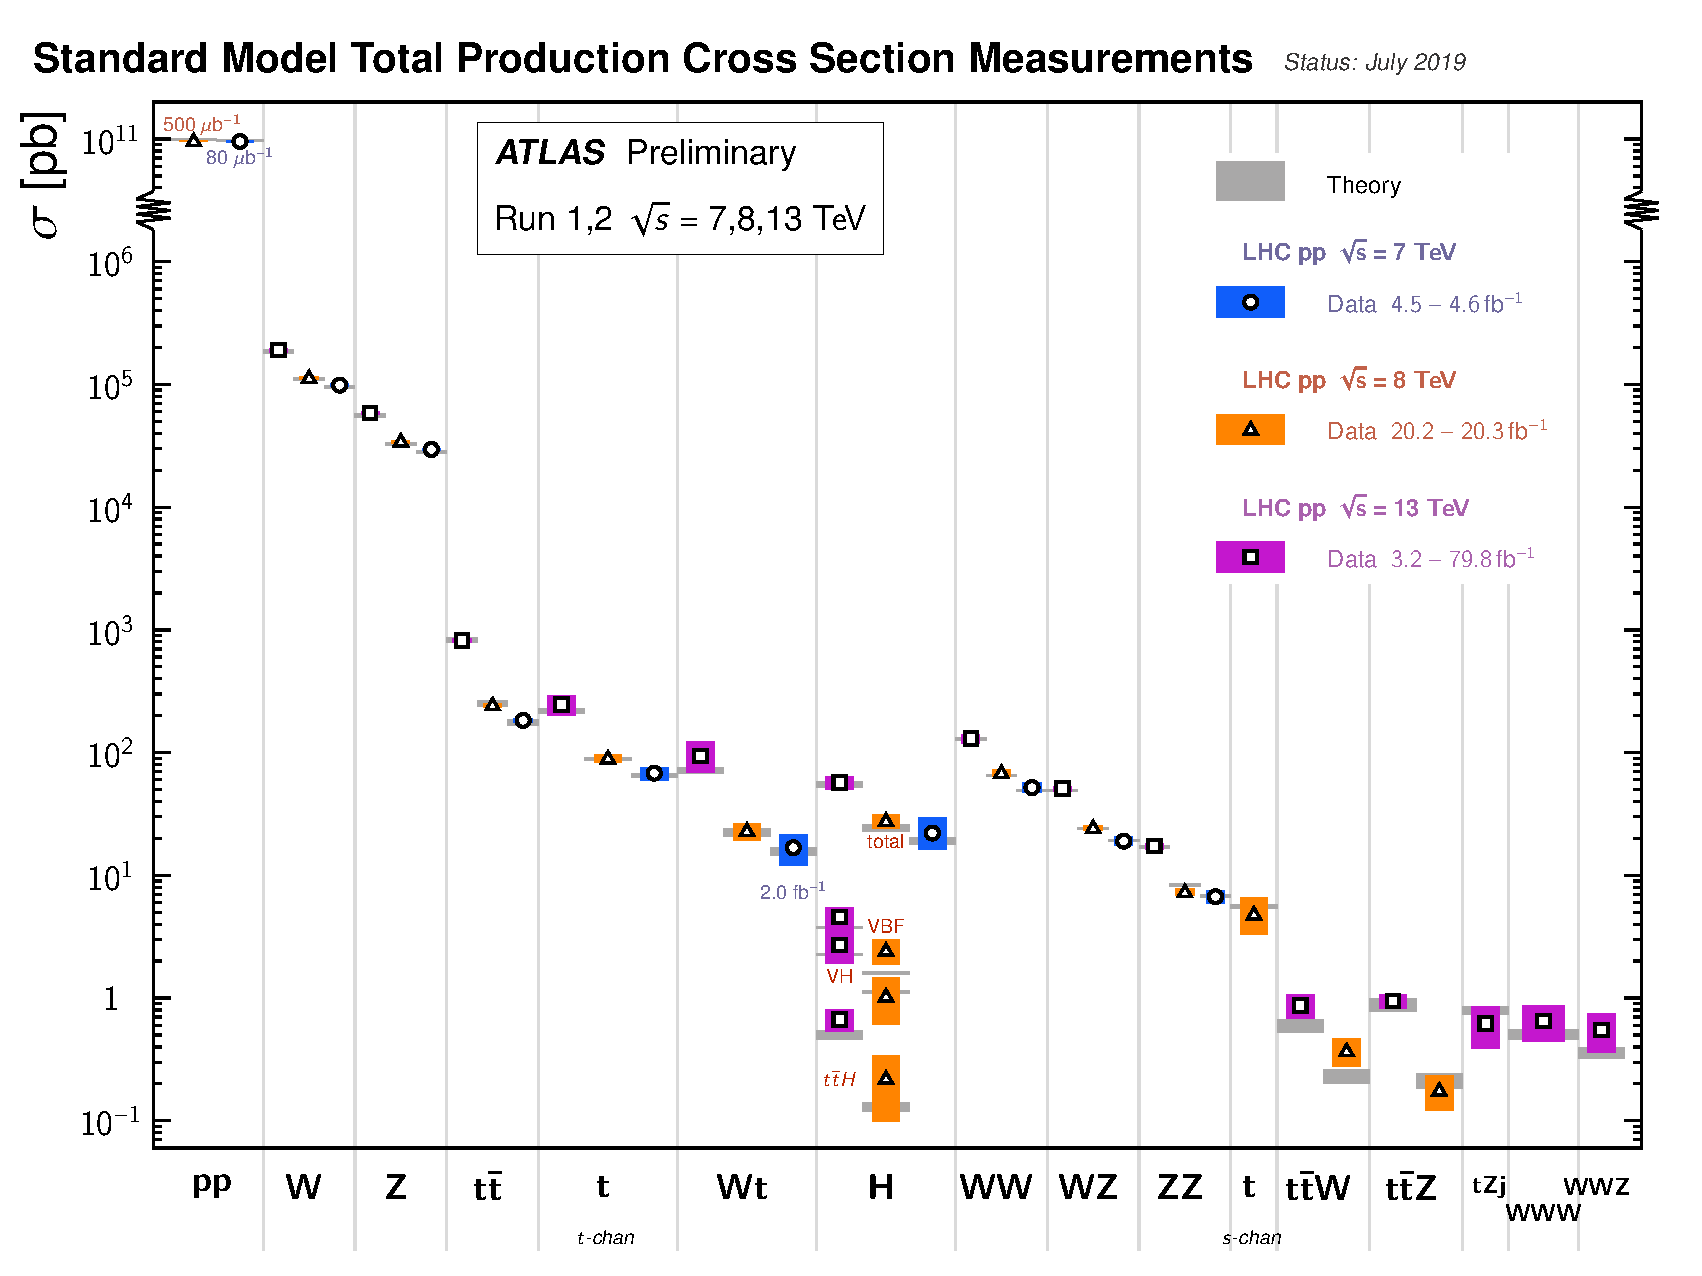
\includegraphics[width=0.75\textwidth]{figures/chapter1/sm_final/sm_xsec_summary}
        \caption{
            Summary of several Standard Model total production cross section measurements,
            corrected for branching fractions, compared to the corresponding theoretical expectations. 
        }
        \label{fig:sm_xsec_summary}
    \end{center}
\end{figure}
\begin{figure}[!htb]
    \begin{center}
        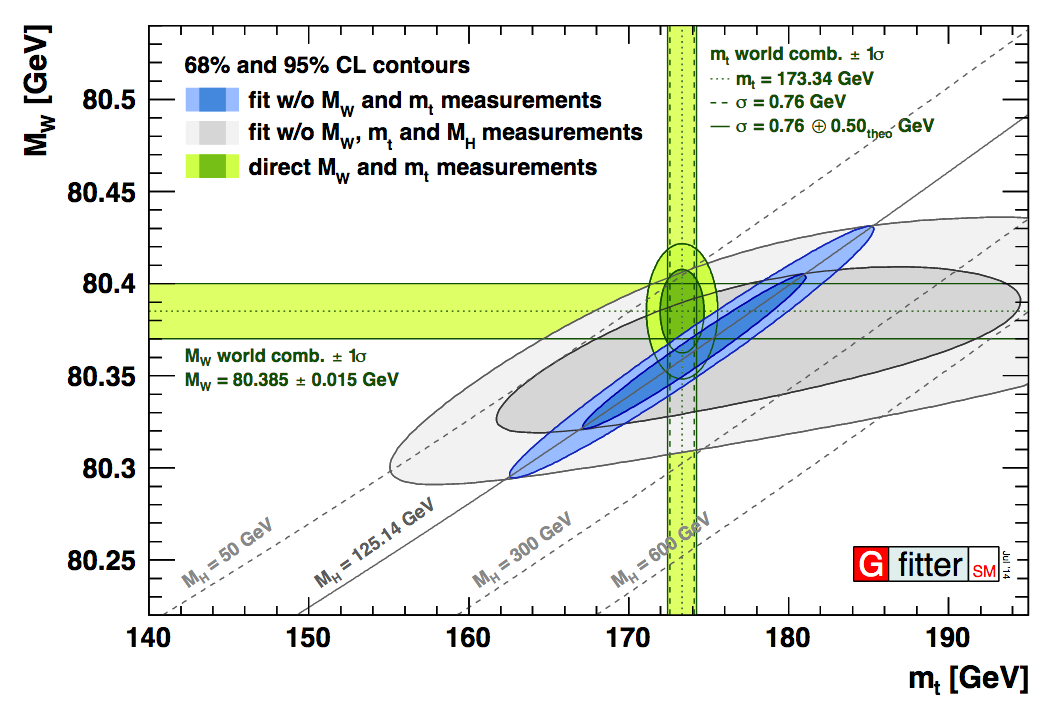
\includegraphics[width=0.65\textwidth]{figures/chapter1/sm_final/mw_vs_mt_indirect}
        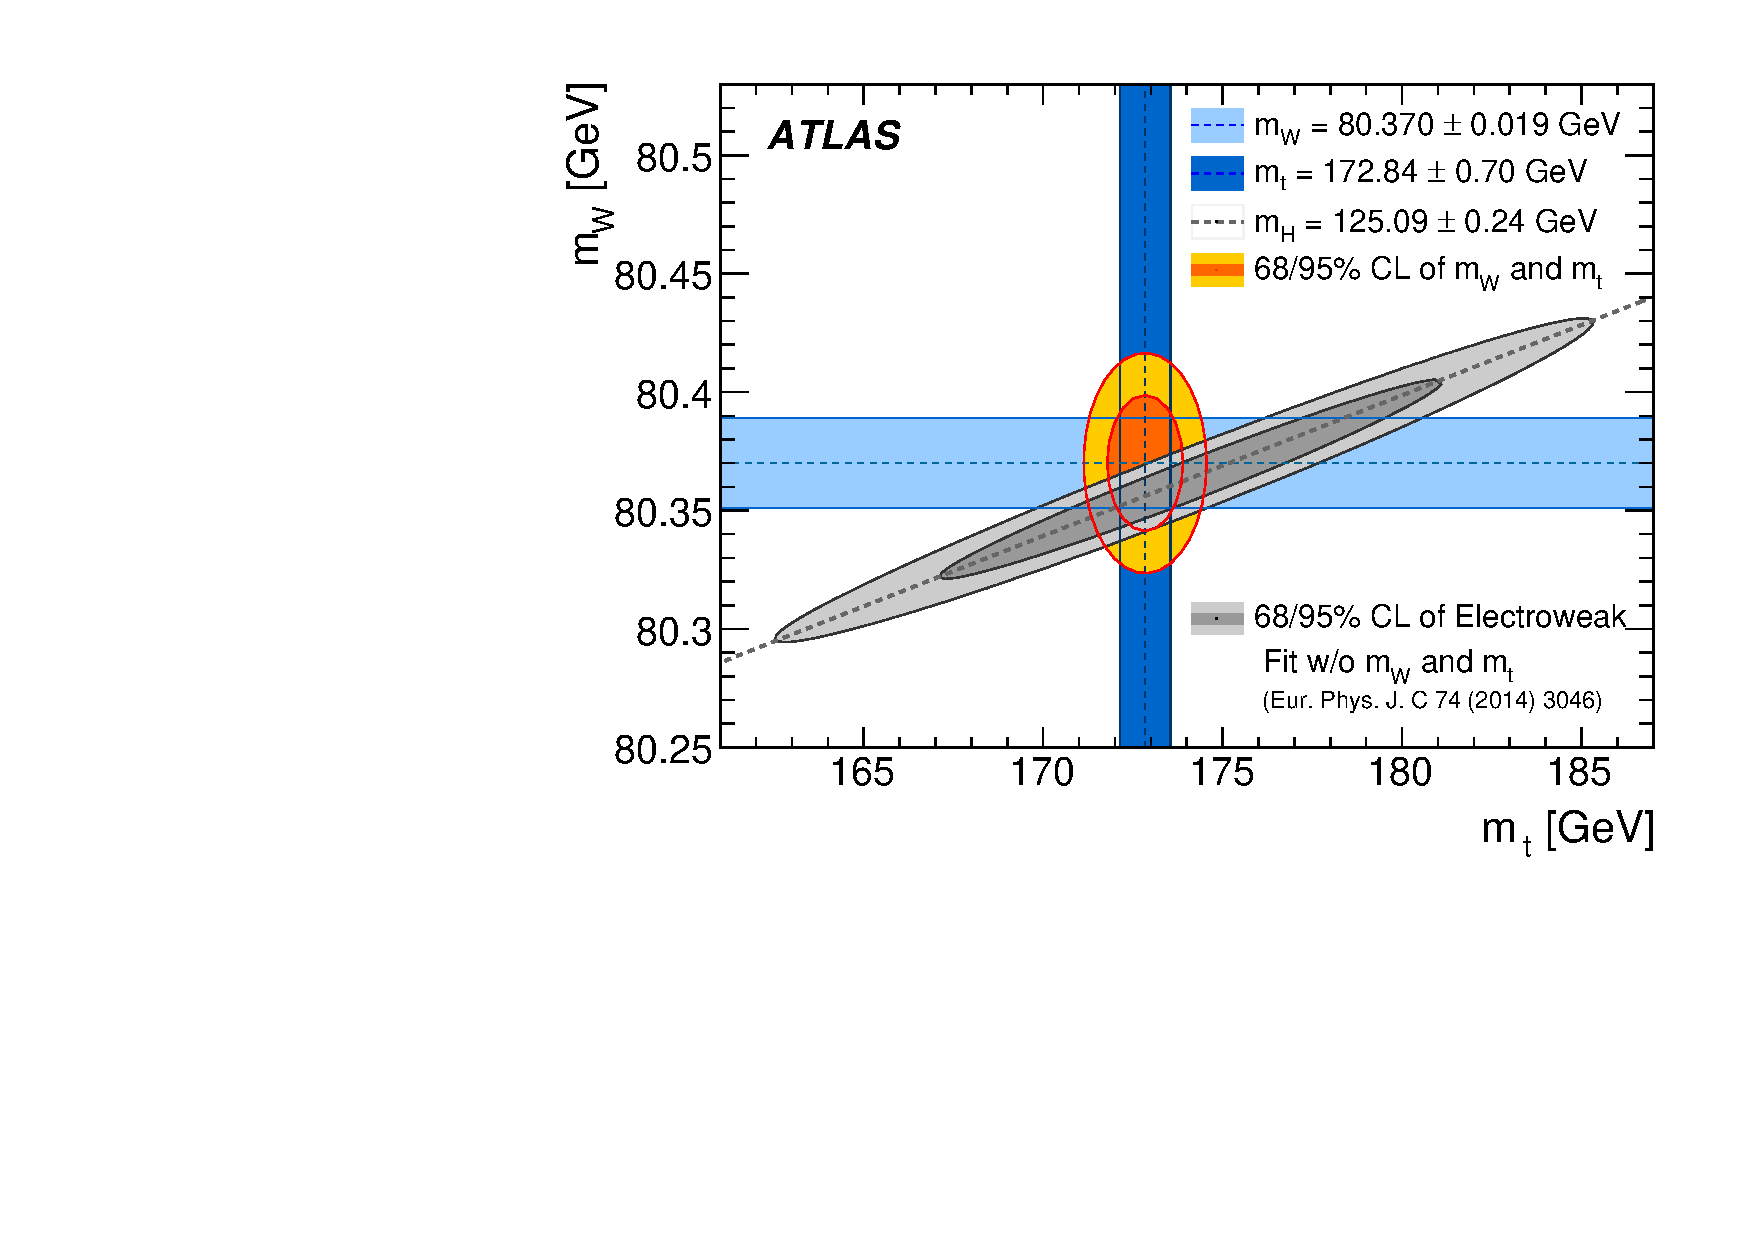
\includegraphics[width=0.69\textwidth]{figures/chapter1/sm_final/atlas_w_boson_mass_mw_mt}
        \caption{
            Contours at 68\% and 95\% CL obtained from scans of $M_W$ versus $m_{\text{top}}$,
            for the global electroweak fits in comparison to the direct measurements.
            \textit{\textbf{Top}}: Including Higgs boson mass measurements in the indirect fit~\cite{HMassATLAS,HMassCMS} (blue)
                or excluding them (grey). From Ref.~\cite{GFitter}.
            \textit{\textbf{Bottom}}: Including the latest precision $W$-boson mass measurement from the ATLAS
                experiment. From Ref.~\cite{ATLASWMass}.
%            for the global electroweak fit including the Higgs boson mass ($m_h$) measurements~\cite{HMassATLAS,HMassCMS} (blue)
%            and excluding the $m_h$ measurements (grey), as compared t the direct
%            measurements of these quantities (green bands and ellipses).
%            From Ref.~\cite{GFitter}.
        }
        \label{fig:mw_mt_scan}
    \end{center}
\end{figure}

With the discovery a Higgs boson like particle with a mass at 125\,GeV in 2012~\cite{HDiscoveryATLAS,HDiscoveryCMS},
the final piece of the SM described by Equation~\ref{eq:sm_lagrangian} is potentially found.
The 2012 Higgs discovery meant the start of a very long experimental program, focused
on studying this new particle and confirming its role as being the fundamental scalar boson, $\phi$,
appearing in the SM.

It should be stressed that the terms associated with the Higgs potential appearing in the SM
Lagrangian, given by Equation~\ref{eq:higgs_potential}, are by no means fundamental.
They do not have to appear in this way.
The terms appearing in Equation~\ref{eq:higgs_potential} take the form they do since they
could lead to masses for the fermions and gauge bosons.
There is no fundamental symmetry motivating their precise form.
The BEH mechanism is inspired by that of super-conductivity, in which the formation composite (i.e. not elementary)
scalar particles --- the Cooper pairs --- occurs.
%The BEH mechanism is inspired by the formation of composite (i.e. not elementary) scalar particles
%appearing in super-conductivity (Cooper pairs).
The fact that the same type of phase transition should describe the generation of masses for
the elementary particles of the SM, and that it should presuppose the existence of an \textit{elementary}
scalar boson, was simply left as one of the last open questions of the SM.
In a sense, the truth of the form underlying Equation~\ref{eq:higgs_potential} was not important to BEH.
The more important takeaway was that there \textit{could} be a mechanism by which the SM particles acquired
mass without disrupting the fundamental gauge structure of the SM that had already held up to experimental scrutiny.
%In a certain sense, this is reflected by the fact that BEH were awarded the Nobel prize only \textit{after} the discoveries of the ATLAS and CMS experiments
%in 2012, whereas GWS were awarded theirs several years \textit{before} the experimental verification of
%the existence of the $W$ and $Z$ bosons.

It is then up to the experiments to verify that the 125\,GeV scalar boson discovered in 2012
is responsible for the BEH mechanism as described in Section~\ref{sec:higgs_description}.
The form of the Higgs potential as defined in Equation~\ref{eq:higgs_potential} makes
very clear predictions on the form and strengths of the couplings to the known fundamental particles:
the gauge bosons and fermions, with couplings to the Higgs predicted to take the forms
of Equations~\ref{eq:higgs_gauge_couplings} and \ref{eq:higgs_fermion_coupling}, respectively.
It is then up to the ATLAS and CMS experiments to verify that the new particle couples
to these `old' particles just as predicted.
The coupling strengths also dictate the Higgs decay rates into specific SM particles, as indicated
in Figure~\ref{fig:higgs_br_sm}.
Any deviation with respect to the SM-predicted values in the measurement of the Higgs decay branching ratios, or
in the values of the fermion or gauge coupling strengths and their dependence on the
particle masses, would indicate that the particle discovered in 2012 is not the Higgs boson as predicted
in the SM.

All of the measurements of the properties of the 125 GeV particle
made by the ATLAS and CMS experiments are so far in fairly good agreement with the SM prediction
of a $m_h = 125$ GeV Higgs boson~\cite{HProp0,HProp1,HProp2,HProp3,HProp4,HProp5,HProp6,HProp7,HProp8}.
The agreement with the SM prediction, over a wide variety of measurements, is illustrated in
Figure~\ref{fig:higgs_measurements} which shows the measurements of the fermion and gauge
couplings and of the cross-sections of the leading Higgs production mechanisms and decay
branching ratios.
Within the precision of these measurements, the SM is fully supported by the experiments
and it appears as though the particle discovered in 2012 is in fact the particle as predicted
by BEH.

\begin{figure}[!htb]
    \begin{center}
        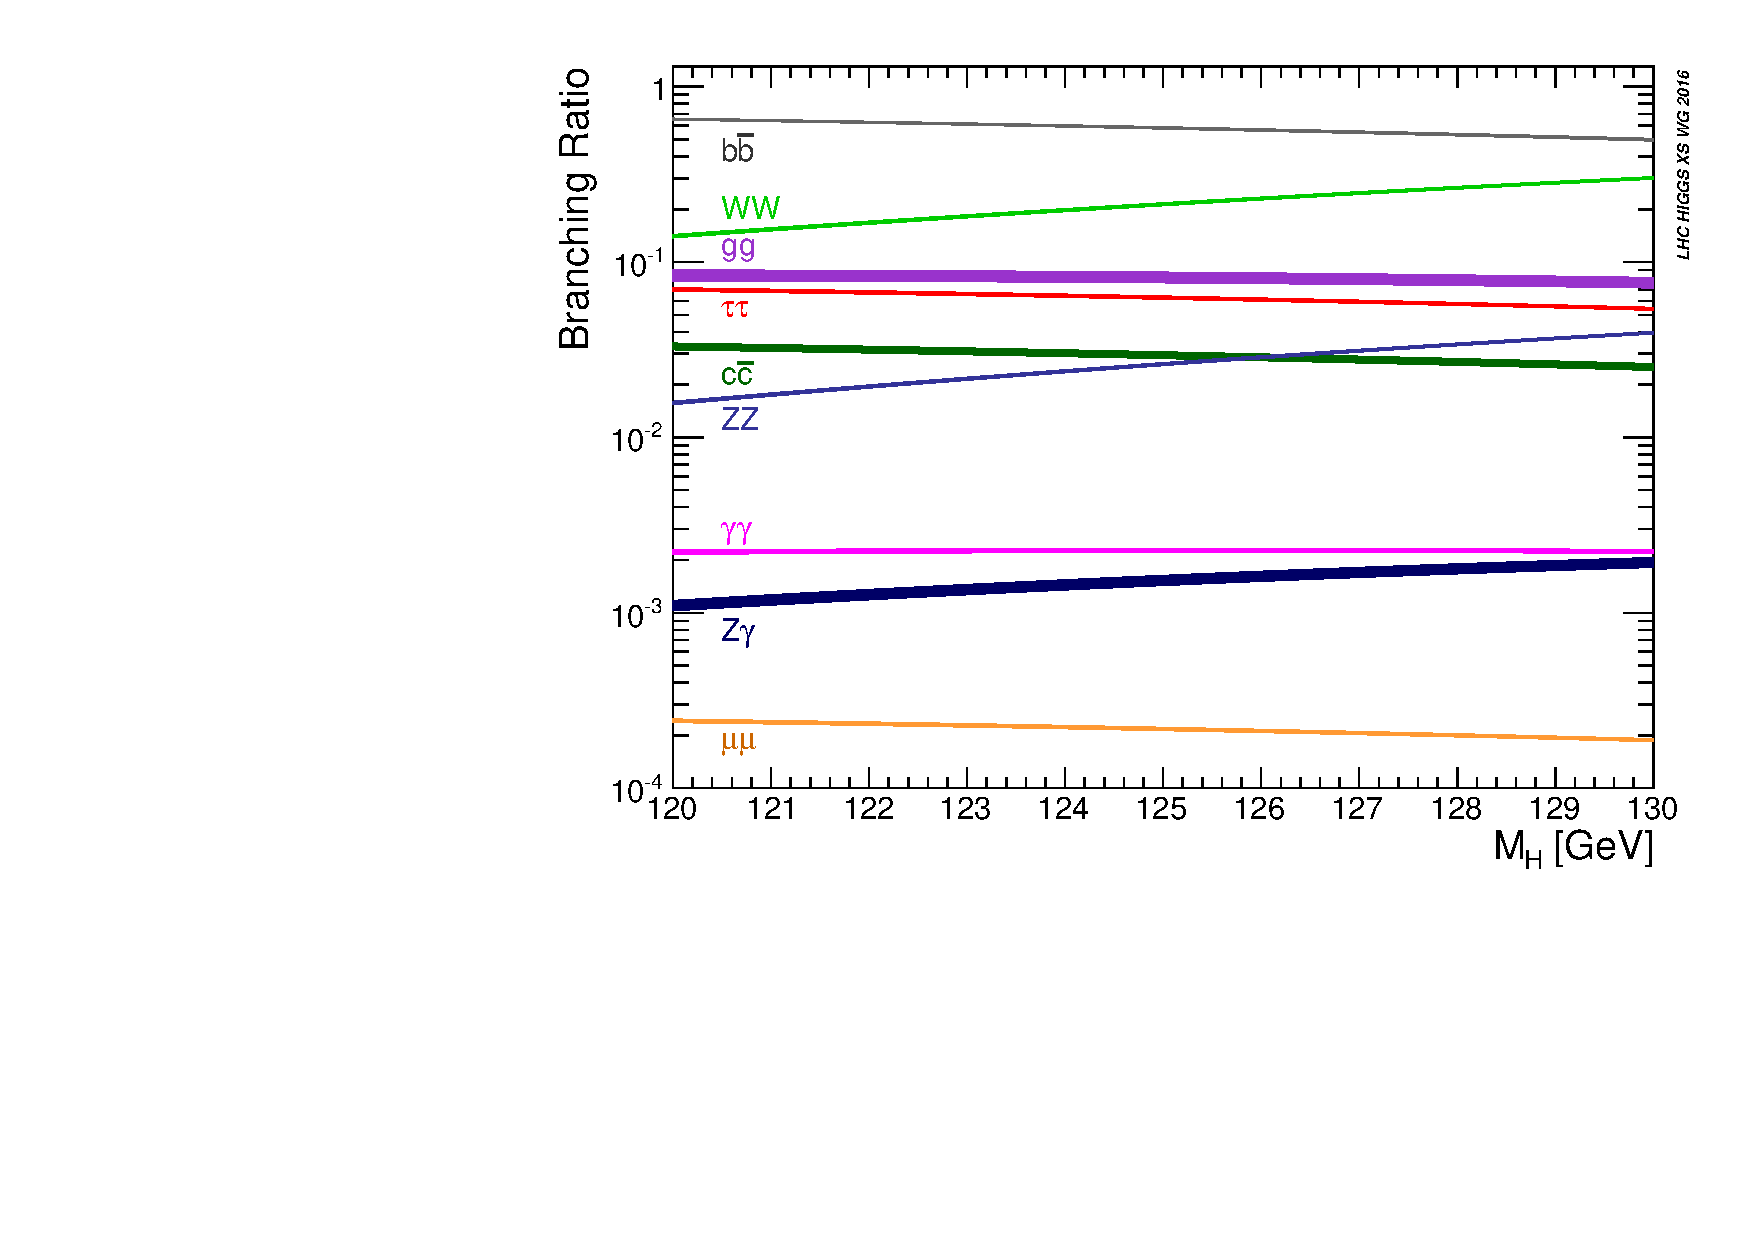
\includegraphics[width=0.6\textwidth]{figures/chapter1/sm_final/higgs_br_sm}
        \caption{
            Predicted branching ratios for an SM-like Higgs boson with $m_{h} = 125\,\GeV$.
        }
        \label{fig:higgs_br_sm}
    \end{center}
\end{figure}

\begin{figure}[!htb]
    \begin{center}
        \raisebox{1cm}{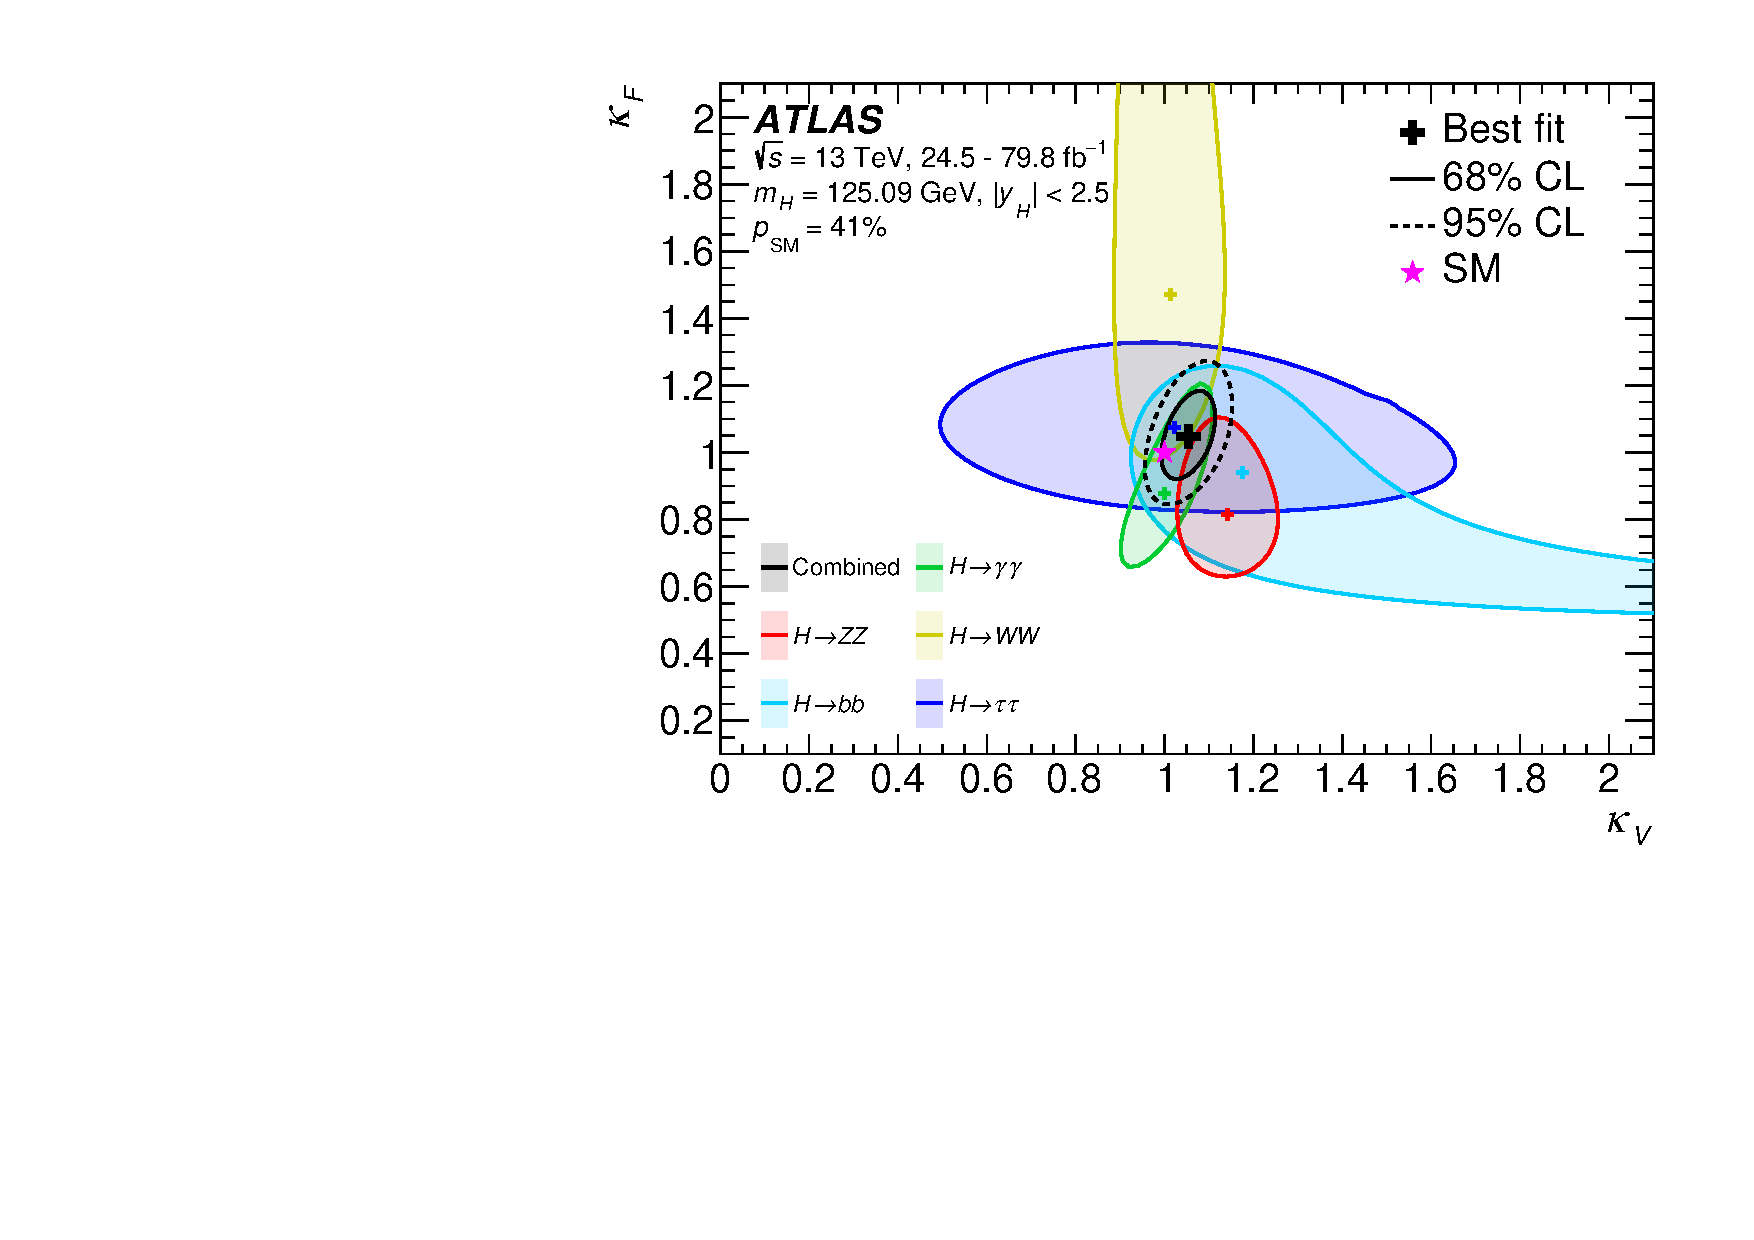
\includegraphics[width=0.49\textwidth]{figures/chapter1/sm_final/higgs_kappa_v_f}}
        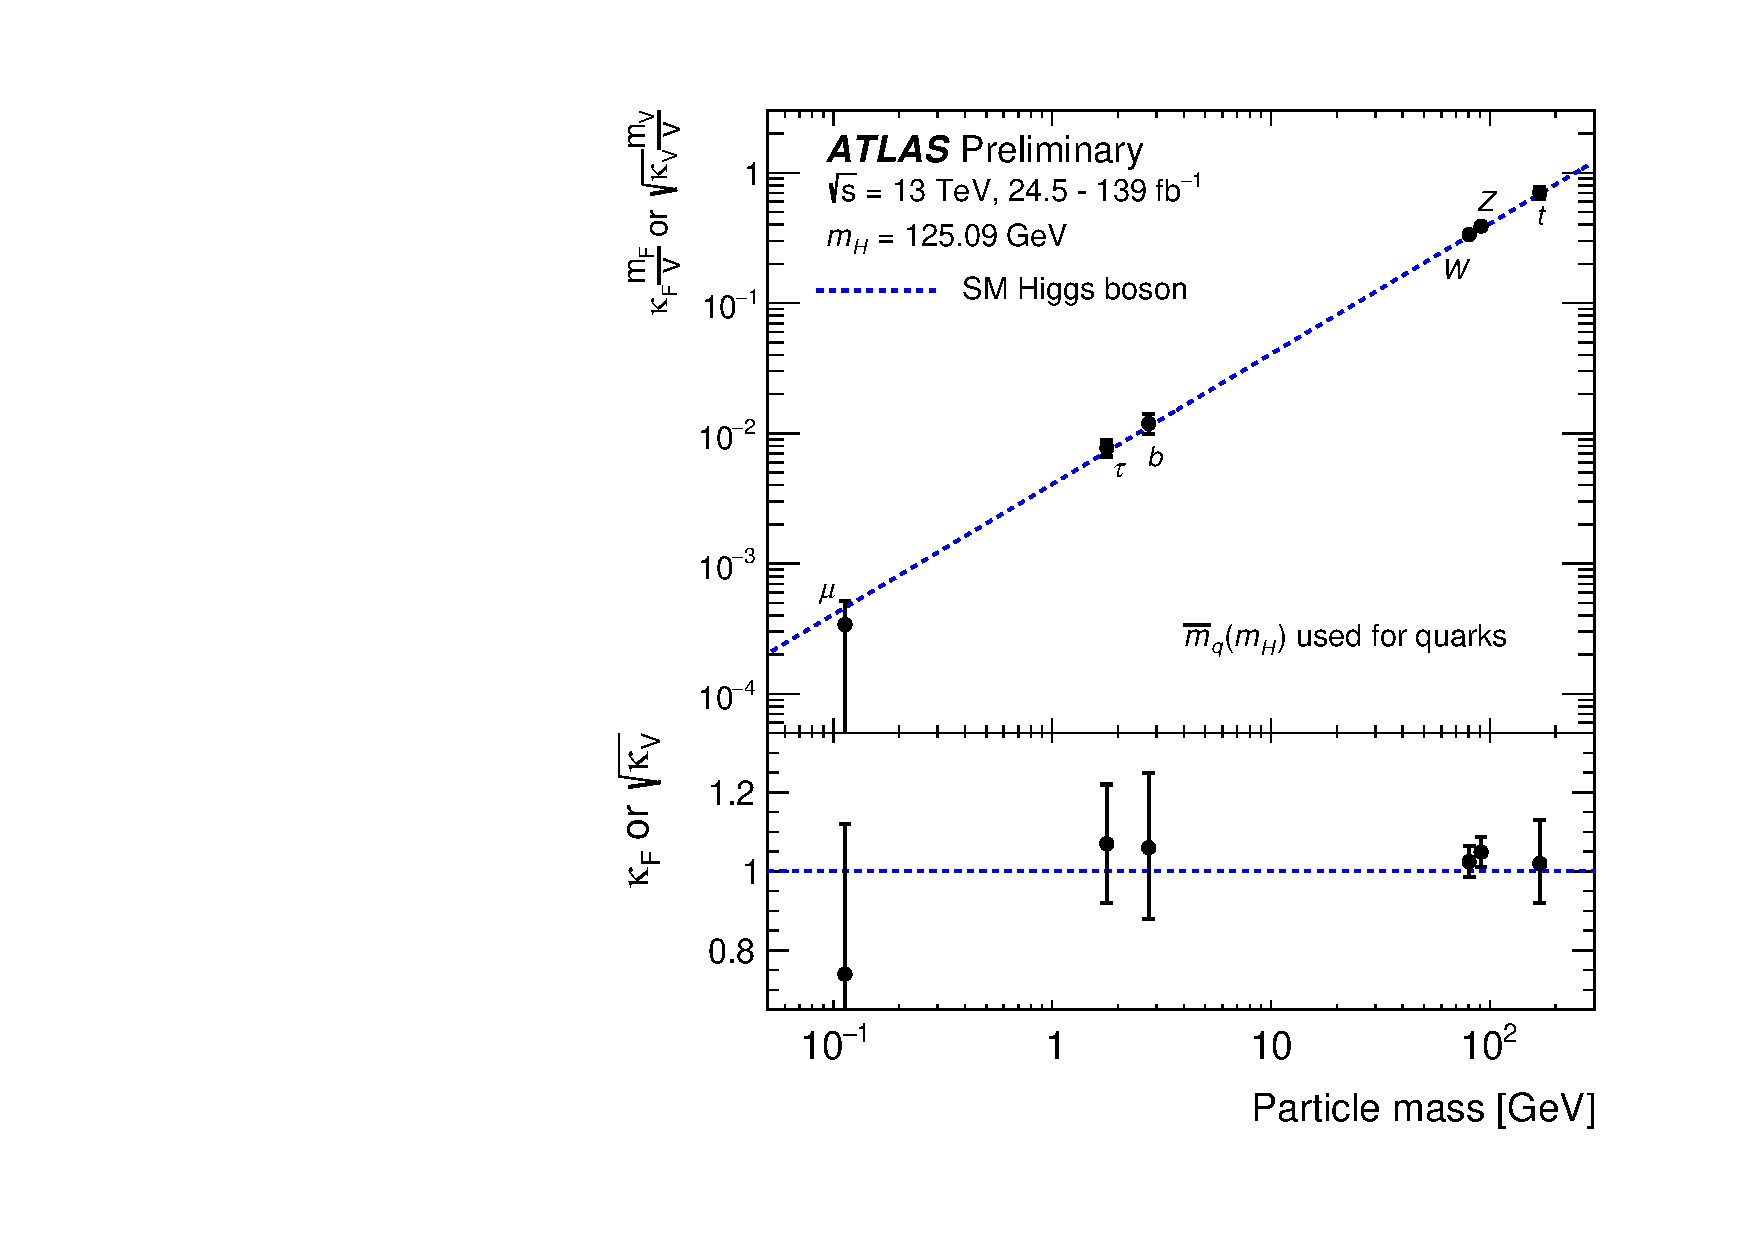
\includegraphics[width=0.49\textwidth]{figures/chapter1/sm_final/higgs_kappa_vs_mass}
        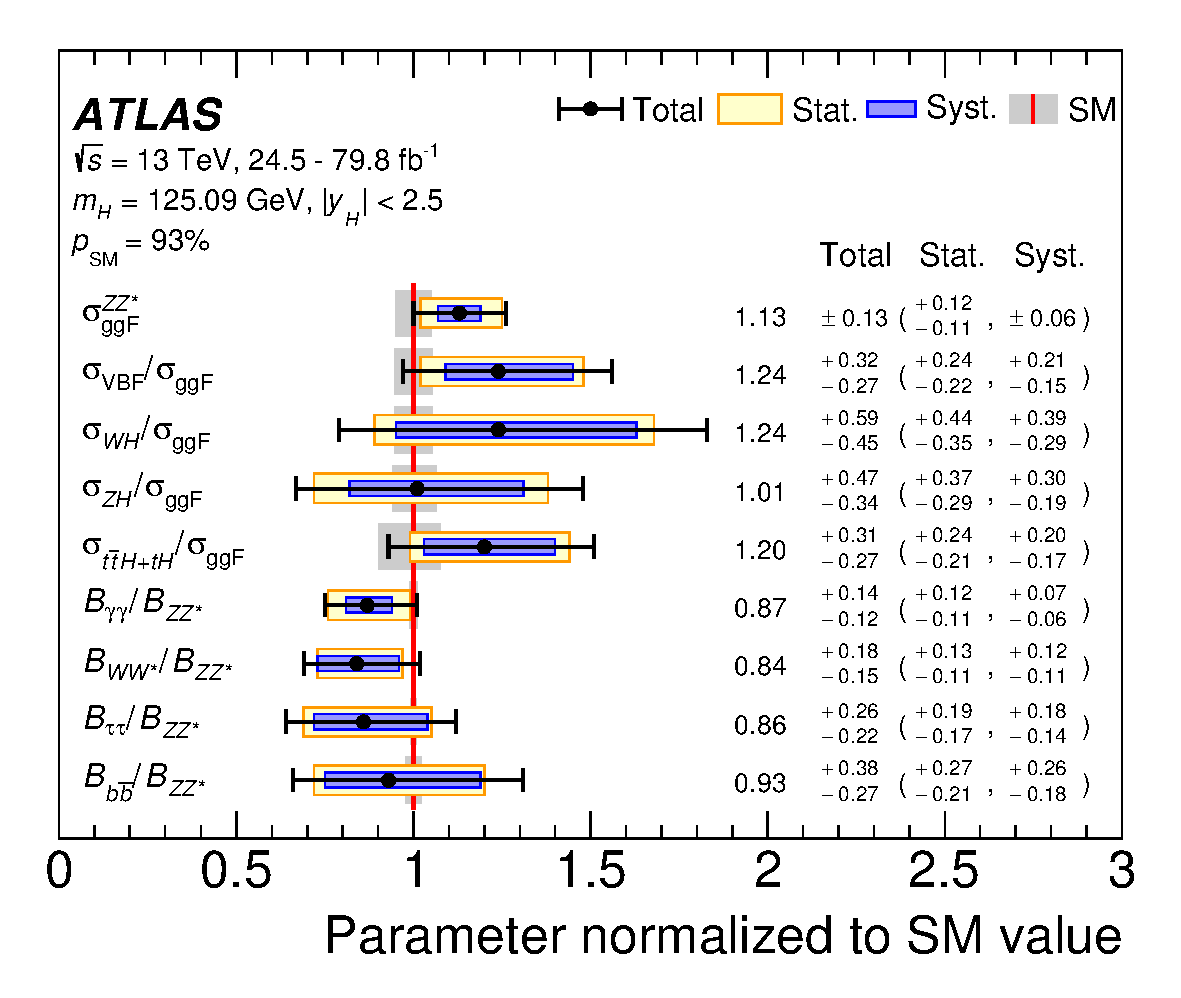
\includegraphics[width=0.49\textwidth]{figures/chapter1/sm_final/higgs_prod_and_br}
        \caption{
            Higgs precision measurements of couplings to SM particles.
            Figures from Ref.~\cite{HiggsProps}.
            \textit{\textbf{Left}}: Combined measurement of fermion and gauge-boson Higgs coupling modifiers, $\kappa_f$
                and $\kappa_V$ (assumed to be universal across fermion and gauge-boson species in the result pictured).
                Values of $\kappa_f$ or $\kappa_V$ equal to 1 correspond to the SM prediction for the Higgs' couplings to
                these particles.
            \textit{\textbf{Right}}: Measured values of the Higgs fermion and gauge-boson coupling parameters
                as a function of the fermion and gauge-boson masses.
                The blue dashed line shows the SM prediction (Equations~\ref{eq:higgs_gauge_couplings} and \ref{eq:higgs_fermion_coupling}).
            \textit{\textbf{Bottom}}: Measurements of Higgs production cross sections and (relative) decay branching ratios.
        }
        \label{fig:higgs_measurements}
    \end{center}
\end{figure}

In addition to the Higgs couplings to the SM fermions and gauge bosons, the SM Lagrangian
predicts terms describing the Higgs \textit{self}-couplings.
These terms are described by the $\lambda$ parameter in Equation~\ref{eq:higgs_potential}
and appearing in Table~\ref{tab:sm_content_EWSB}.
The Higgs self-coupling parameter $\lambda$ has a value predicted by the SM, as seen in 
Equation~\ref{eq:higgs_self_couplings}, which is fixed by the Higgs boson mass.
The parameter $\lambda$ is directly responsible for providing the structure of the Higgs potential,
indicated by Equation~\ref{eq:higgs_potential_self_int}, and therefore plays a fundamental
role in EWSB.
Measuring how the 125\,GeV Higgs boson couples and decays to the SM fermions and gauge bosons,
then, is only a necessary requirement for confirming that the particle is the one predicted by
the SM: it is not sufficient.
To truly confirm that the 125\,GeV boson is indeed that predicted by the SM, and that EWSB
is described by the BEH mechanism, the Higgs self-coupling parameter will have to be measured
experimentally and confirmed to take its predicted value given by Equation~\ref{eq:higgs_self_couplings}.

Direct measurement of $\lambda$ proceeds only through the observation of events in which Higgs bosons
are produced in pairs.
At the LHC, this process occurs predominantly via gluon-gluon fusion through the two diagrams illustrated
in Figure~\ref{fig:hh_feynman}.
The triangle and box diagrams shown in Figure~\ref{fig:hh_feynman} represent destructively interfering amplitudes.
As a result, the cross-sections associated with the production of Higgs boson pairs is exceedingly low
and statistically significant observation of this process is not expected to occur until
near the end of the lifetime of the LHC.
The study of Higgs boson pairs is the subject of the analysis to be presented in Chapter~\ref{chap:search_hh}.

\begin{figure}[!htb]
    \begin{center}
        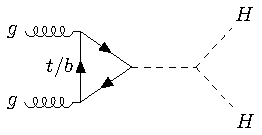
\includegraphics[width=0.7\textwidth]{figures/search_hh/feynman_diagrams/fdiagram_triangle}
        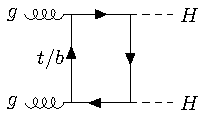
\includegraphics[width=0.55\textwidth]{figures/search_hh/feynman_diagrams/fdiagram_box}
        \caption{
            Representative Feynman diagrams that contribute at leading order in QCD to the non-resonant
            production of Higgs boson pairs.
            {\textbf{\textit{Top}}}: The `triangle' diagram, sensitive to the Higgs self-coupling, $\lambda$.
            {\textbf{\textit{Bottom}}}: The `box' diagram, sensitive to the (squared) Yukawa couplings to the third generation
            fermions entering the loop.
        }
        \label{fig:hh_feynman}
    \end{center}
\end{figure}

%%%%%%%%%%%%%%%%%%%%%%%%%%%%%%%%%%%%%%%%%%%%%%%%%%%%%%%%%%%%%%%%%%%%%%%%%%%%%%%%%
%%%%%%%%%%%%%%%%%%%%%%%%%%%%%%%%%%%%%%%%%%%%%%%%%%%%%%%%%%%%%%%%%%%%%%%%%%%%%%%%%
%%%%%%%%%%%%%%%%%%%%%%%%%%%%%%%%%%%%%%%%%%%%%%%%%%%%%%%%%%%%%%%%%%%%%%%%%%%%%%%%%
%
% SHORTCOMINGS
%
%%%%%%%%%%%%%%%%%%%%%%%%%%%%%%%%%%%%%%%%%%%%%%%%%%%%%%%%%%%%%%%%%%%%%%%%%%%%%%%%%
%%%%%%%%%%%%%%%%%%%%%%%%%%%%%%%%%%%%%%%%%%%%%%%%%%%%%%%%%%%%%%%%%%%%%%%%%%%%%%%%%
%%%%%%%%%%%%%%%%%%%%%%%%%%%%%%%%%%%%%%%%%%%%%%%%%%%%%%%%%%%%%%%%%%%%%%%%%%%%%%%%%
\FloatBarrier
\subsection{Perceived Shortcomings of the Standard Model and Open Questions}
\label{sec:sm_shortcomings}

Despite the impressive results and predictive power of the SM illustrated in the previous
section, the SM is unable to provide a complete picture of what we now consider the observed
Universe.
A few items that are clearly not explained within the framework of the SM are described below.
%A few items that are clearly not explainable under the framework of the SM are described below.
Chapter~\ref{chap:bsm} goes on to introduce an extension to the SM that provides explanations
for many of these short comings of the SM.

\begin{description}
    \item[] \textbf{Existence of Dark Matter (DM) and Dark Energy (DE)} \\
        Most of the experimental evidence that we currently have that supports the notion that
        physics beyond the SM (BSM) exists comes not from collider-based particle physics experiments,
        but from astrophysical observations.
        Astrophysical observations suggest that the majority of the matter content of the Universe
        is composed of a non-luminous, weakly interacting type of matter referred to as `Dark Matter' (DM)
        and that the expansion of the Universe is accelerating, perhaps due to presence of
        `Dark Energy' (DE)~\cite{Davis:2014csa,PlanckCollab}.
        There has not yet been experimental proof of the particle nature of DM, but
        many theories suggest that it fall under the class of `Weakly Interacting Massive Particle' (WIMPs), i.e. that it be `WIMP-like'.
        The particle nature of DE is completely unknown and without a fundamental description.
    \item[] \textbf{Massive Neutrinos} \\ The observation of neutrino oscillations~\cite{Fukuda:1998mi} provides evidence
        in support of neutrinos having nonzero masses. This directly contradicts the massless neutrino hypothesis of the SM.
    \item[] \textbf{Matter-Antimatter Asymmetry} \\
        The only parameter in the SM that allows for CP violation is the CP-violating phase in the CKM matrix,
        which is unable to account for the amount of CP violation needed to account for the
        observed asymmetry in the amount of matter over antimatter in the Universe.
        Additional CP violating effects are necessary to account for this observed asymmetry and should be relevant
        to early-Universe cosmology~\cite{Sakharov_1991}.
    \item[] \textbf{The Hierarchy Problem} \\
        The Hierarchy Problem refers to the fact that the electroweak sector, through the scalar Higgs boson,
        is sensitive to high energy cut-off scales nearing the Planck Mass, $M_{P} \approx 10^{18}--10^{19}$\,GeV.
        This is evident when computing the higher-order corrections to the Higgs mass,
        \begin{align*}
            m_h^2 = m_{h,\,0}^2 + \Delta m_h^2,
        \end{align*}
        which are found to be quadratically divergent due to the fact that the Higgs is not protected by any fundamental
        internal symmetries:
        %\vspace{-1.2cm}
        \begin{align}
            \Delta m_h^2 = -\frac{ |y_f|^2 }{16 \pi^2} \left[ 2 \Lambda^2  + \mathcal{O} \left( m_f^2 \ln \left( \frac{\Lambda}{m_f} \right) \right) \right],
            \label{eq:higgs_divergence}
        \end{align}
        where $y_f$ is the fermion Yukawa coupling, $m_f$ is the associated fermion mass, and $\Lambda$ is the
        ultra-violate cut-off scale.
        Similar terms also appear for the SM gauge bosons, resulting in their own contributions like Equation~\ref{eq:higgs_divergence}, but given the near-unity Yukawa coupling of the top-quark,
        the divergence is most evident from the top-quark loop contributions to $\Delta m_h^2$, such as that shown in Figure~\ref{fig:higgs_mass_correction}.
        %the divergence is most sensitive to the fermion terms appearing in the above via $y_t$.
        \begin{figure}[!htb]
        \hspace{1.8cm}
        \begin{minipage}{0.8\textwidth}
            \begin{center}
                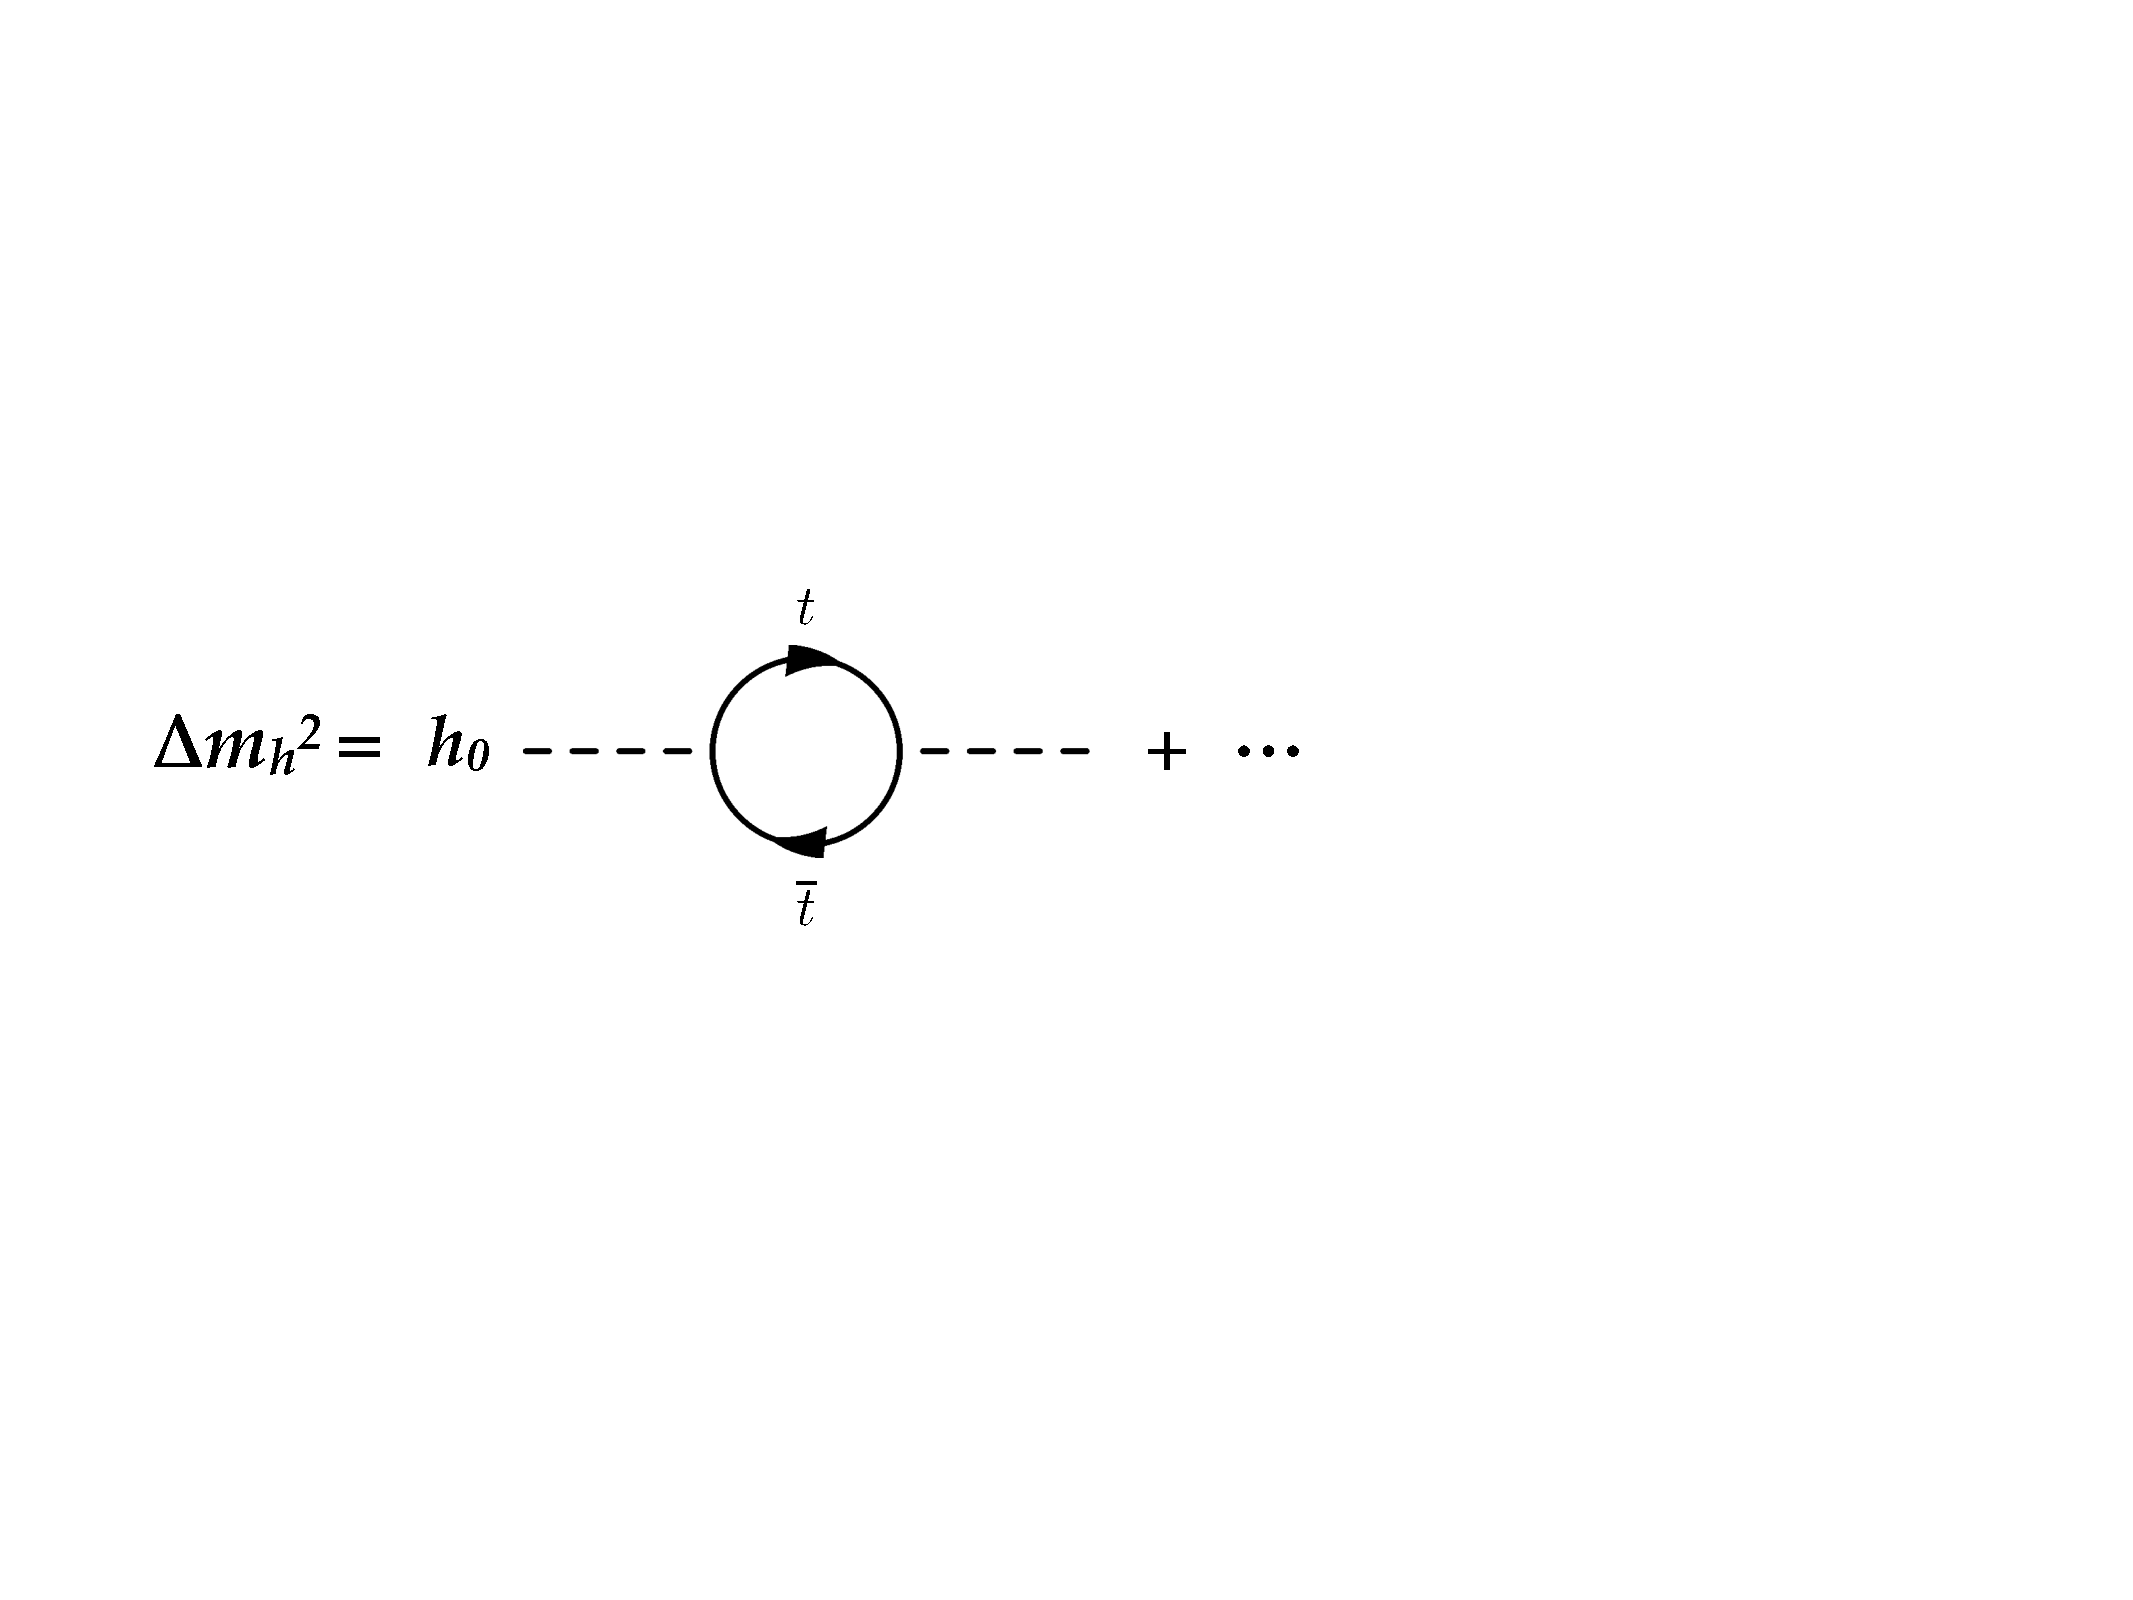
\includegraphics[width=0.6\textwidth]{figures/higgs_corr/higgs_mass_correctionsPDF}
                \caption{
                    Top-quark loop contribution to the higher-order computation of the Higgs mass that
                    leads to unregulated divergent terms such as Equation~\ref{eq:higgs_divergence}.
                }
                \label{fig:higgs_mass_correction}
            \end{center}
        \end{minipage}
        \end{figure}
        The apparent contradiction that the electroweak scale at which the Higgs boson is experimentally known to exist
        should also be unavoidably sensitive to $M_P$, attempting to drive the Higgs boson mass to values 16 orders
        of magnitude larger than the measured one,
        is at the heart of the Hierarchy Problem.
        The high energy scales at which SM calculations fail are typically assumed to be the scales
        at which new physics arise and take over as a more complete description of natural pheneomena.
        That the Higgs boson is apparently driven to these scales motivates the arguments in favor
        of their being new physics at or near the electroweak scale which act to cancel the quadratically
        divergent terms appearing in the Higgs mass corrections.
        That cancellations of terms on the order of $10^{30}$ ($\Lambda^2$) should be possible introduces the
        philosophical concerns of \textit{naturalness}, which ponder whether or not Nature is such
        that the additional sources of high energy physics --- not accounted for by the SM --- can conspire in such a way as to
        allow for such perfectly fine-tuned cancellation.
\end{description}

%eq:higgs_potential



%\section{Particles and Forces}
%
%Here we introduce the SM particle content and provide a description of the interactions that
%link the particles together.
%
%
\begin{table}[!htb]
    \caption{
        The particle content of the SM and their transformation
        properties under the SM gauge groups, prior to electroweak symmetry breaking.
        The representations of each of the gauge groups are shown in the three-right
        columns. The \Uone symmetry of weak-hypercharge transformations is one-dimensional
        and the column gives the weak-hypercharge $\mathcal{Y}$ associated with each
        field. For \SUthree and \SUtwo, $\mathbf{1}$ refers to the field belonging to
        the associated singlet representation, $\mathbf{2}$ to the doublet representation,
        $\mathbf{3}$ to the triplet representation, and $\mathbf{8}$ to the octet representation.
    }
    \begin{center}
        \begin{tabularx}{0.96\textwidth}{m{1em} c c c c c c }
        \toprule
        \hline
        & Field Label & Content & Spin & \Uone~($\mathcal{=Y}$) & \SUtwo & \SUthree \\
        \hline
        \rotatebox{90}{\hspace{-0.1cm}\textbf{Quarks} } 
         &   \makecell{\fieldQi \\ \fieldUri \\ \fieldDri} % FIELD
         &   \makecell{ (\fieldUl, \fieldDl), (\fieldCl, \fieldSl), (\fieldTl, \fieldBl) \\ \fieldUr \\ \fieldDr}% CONTENT
         &   \makecell{ $1/2$ \\ $1/2$ \\ $1/2$} % SPIN
         &   \makecell{ $1/6$ \\ $2/3$ \\ $-1/3$}% U(1)
         &   \makecell{ $\mathbf{2}$ \\ $\mathbf{1}$ \\ $\mathbf{1}$}% SU(2)
         &   \makecell{ $\mathbf{3}$ \\ $\mathbf{3}$ \\ $\mathbf{3}$}\\ % SU(3)
        %\cdashline{1-7}
        \rotatebox{90}{\hspace{-0.1cm}\textbf{Leptons} }
         &   \makecell{\fieldLi \\ \fieldEri} % FIELD
         &   \makecell{ (\fieldEl, \fieldNuEl), (\fieldMul, \fieldNuMul), (\fieldTaul, \fieldNuTaul) \\ \fieldEr, \fieldMur, \fieldTaur}% CONTENT
         &   \makecell{ $1/2$ \\ $1/2$ }% SPIN
         &   \makecell{ $1/2$ \\ $-1$ }% U(1)
         &   \makecell{ $\mathbf{2}$ \\ $\mathbf{1}$ }% SU(2)
         &   \makecell{ $\mathbf{1}$ \\ $\mathbf{1}$ } \\ % SU(3)
        \midrule
        \rotatebox{90}{\textbf{\stackanchor{Gauge}{Fields}} }
         &   \makecell{\fieldB \\ \fieldW \\ \fieldG } % FIELD
         &   \makecell{ \fieldB \\ (\fieldWone, \fieldWtwo, \fieldWthree) \\ \fieldG$_a$, $a\in[1,..,8]$ }% CONTENT
         &   \makecell{ $1$ \\ $1$ \\ $1$} % SPIN
         &   \makecell{ $0$ \\ $0$ \\ $0$}% U(1)
         &   \makecell{ $\mathbf{1}$ \\ $\mathbf{3}$ \\ $\mathbf{1}$}% SU(2)
         &   \makecell{ $\mathbf{1}$ \\ $\mathbf{1}$ \\ $\mathbf{8}$}\\ % SU(3)
        \midrule
        \rotatebox{90}{\textbf{\stackanchor{Higgs}{Field}}} 
         &   \makecell{\fieldPhi } % FIELD
         &   \makecell{ (\fieldPhip, \fieldPhizero) }% CONTENT
         &   \makecell{ $0$  } % SPIN
         &   \makecell{ $1/2$  }% U(1)
         &   \makecell{ $\mathbf{2}$ }% SU(2)
         &   \makecell{ $\mathbf{1}$ }\\ % SU(3)
        \hline
        \bottomrule
        \end{tabularx}
    \end{center}
    \label{tab:sm_content}
\end{table}

%
\begin{table}[!htb]
    \caption{
        The particle content of the SM after the process of
        electroweak symmetry breaking.
    }
    \begin{center}
        \begin{tabularx}{1\textwidth}{m{1em} c c c c }
        \toprule
        \hline
        & Physical Field & Q & Coupling & Mass [GeV] \\
        \hline
        \rotatebox{90}{\hspace{-0.1cm}\textbf{Quarks} } 
            & \makecell{ \quarkU, \quarkC, \quarkT \\ \quarkD, \quarkS, \quarkB} % FIELD
            & \makecell{ $2/3$ \\ $-1/3$ }% Q
            %& \makecell{ $\mathbf{3}$ \\ $\mathbf{3}$ } % SU(3)
            & \makecell{ ($y_i=$) $1\times10^{-5}$, $7\times10^{-3}$, $1$ \\ ($y_i=$) $3\times10^{-5}$, $5\times10^{-4}$, $0.02$ } % Coupling
            & \makecell{ $2\times10^{-3}$, $1.27$, $173$ \\ $4\times10^{-4}$, $0.10$, $4.18$ }\\% Mass
        \rotatebox{90}{\hspace{-0.1cm}\textbf{Leptons} } 
            & \makecell{ \leptonE, \leptonMu, \leptonTau \\ \neutrinoE, \neutrinoMu, \neutrinoTau } % FIELD
            & \makecell{ $-1$ \\ $0$ }% Q
            %& \makecell{ $\mathbf{1}$ \\ $\mathbf{1}$ } % SU(3)
            & \makecell{ ($y_i=$) $3\times10^{-7}$, $6\times10^{-4}$, $0.01$ \\ -- } % Coupling
            & \makecell{ $5\times10^{-4}$, $0.106$, $1.777$ \\ --}\\% Mass
        \midrule
        \rotatebox{90}{\textbf{Bosons} } 
            & \makecell{ \fieldPhoton \\ \fieldZ \\ (\fieldWp, \fieldWm) \\ \fieldG } % FIELD
            & \makecell{ $0$ \\ $0$ \\ $(+1,-1)$ \\ $0$ }% Q
            %& \makecell{ $\mathbf{1}$ \\ $\mathbf{1}$ \\ $\mathbf{1}$ \\ $\mathbf{8}$ } % SU(3)
            & \makecell{ $\alpha_{\text{EM}} \simeq 1/137$ \\ $\sin \theta_{W} \simeq 0.5$ \\ -- \\ $\alpha_s \simeq 0.1$ } % Coupling
            & \makecell{ $0$ \\ $91.2$ \\ $80.4$ \\  $0$}\\% Mass
        \midrule
        \rotatebox{90}{\textbf{Higgs} } 
            & \makecell{ \fieldH } % FIELD
            & \makecell{ $0$ }% Q
            %& \makecell{ $\mathbf{1}$ } % SU(3)
            & \makecell{ $\lambda$, $\mu$ } % Coupling
            & \makecell{ $125.09$ }\\% Mass

         %&   \makecell{ (\quarkUl, \quarkDl), (\quarkCl, \quarkSl), (\quarkTl, \quarkBl) \\ \quarkUr \\ \quarkDr}% CONTENT
         %&   \makecell{ $1/2$ \\ $1/2$ \\ $1/2$} % SPIN
         %&   \makecell{ $\mathbf{2}$ \\ $\mathbf{1}$ \\ $\mathbf{1}$}% SU(2)
         %&   \makecell{ $\mathbf{3}$ \\ $\mathbf{3}$ \\ $\mathbf{3}$}\\ % SU(3)
        %%\cdashline{1-7}
        %rotatebox{90}{\hspace{-0.1cm}\textbf{Leptons} }
         %&   \makecell{\quarkLi \\ \quarkEri} % FIELD
         %&   \makecell{ (\quarkEl, \quarkNuEl), (\quarkMul, \quarkNuMul), (\quarkTaul, \quarkNuTaul) \\ \quarkEr, \quarkMur, \quarkTaur}% CONTENT
         %&   \makecell{ $1/2$ \\ $1/2$ }% SPIN
         %&   \makecell{ $\mathbf{2}$ \\ $\mathbf{1}$ }% SU(2)
         %&   \makecell{ $\mathbf{1}$ \\ $\mathbf{1}$ } \\ % SU(3)
        %midrule
        %rotatebox{90}{\textbf{\stackanchor{Gauge}{Fields}} }
         %&   \makecell{\quarkB \\ \quarkW \\ \quarkG } % FIELD
         %&   \makecell{ \quarkB \\ (\quarkWone, \quarkWtwo, \quarkWthree) \\ \quarkG }% CONTENT
         %&   \makecell{ $1$ \\ $1$ \\ $1$} % SPIN
         %&   \makecell{ $\mathbf{1}$ \\ $\mathbf{3}$ \\ $\mathbf{1}$}% SU(2)
         %&   \makecell{ $\mathbf{1}$ \\ $\mathbf{1}$ \\ $\mathbf{8}$}\\ % SU(3)
        %midrule
        %rotatebox{90}{\textbf{\stackanchor{Higgs}{Field}}} 
         %&   \makecell{\quarkPhi } % FIELD
         %&   \makecell{ (\quarkPhip, \quarkPhizero) }% CONTENT
         %&   \makecell{ $0$  } % SPIN
         %&   \makecell{ $\mathbf{2}$ }% SU(2)
         %&   \makecell{ $\mathbf{1}$ }\\ % SU(3)
        \hline
        \bottomrule
        \end{tabularx}
    \end{center}
    \label{tab:sm_content}
\end{table}



%\subsection{Gauge Theories}

%\subsubsection{The Electroweak Theory}


